


\section{Einleitung}



\begin{frame}
 \frametitle{Einleitung}
  


\begin{itemize}
  \item \pause Spiele als Lernumgebung für AI
\begin{itemize}
  \item \pause 1951: Nimrod
  \item \pause 1995: Vier gewinnt
  \item \pause 1997: Schach
  \item \pause 2016: Go
\end{itemize}
\end{itemize}

\begin{itemize}
  \item \pause AlphaGo
  \item \pause AlphaZero
  \item \pause Großer Rechenaufwand nötig: 5000+ TPUs
\end{itemize}

  
\end{frame}
\begin{frame}
 \frametitle{Zielsetzung}
  


\begin{itemize}
  \item \pause Untersuche mögliche Effizienzsteigerungen
  \item \pause Solide Baseline
  \item \pause Experimentiere mit Vier gewinnt
  \item \pause Evaluiere verschiende neue Ideen
\begin{itemize}
  \item \pause Evolution von Hyperparametern
  \item \pause Self-play im Baumformat
  \item \pause Auxiliary Features
\end{itemize}
\end{itemize}

  
\end{frame}

\section{Grundlagen}




\subsection{Algorithmus}



\begin{frame}
 \frametitle{Monte Carlo tree search (MCTS)}
  


\begin{itemize}
  \item \pause Seit 2006 sehr verbreitet in Computer Go.
  \item \pause Iterativer Baumsuchalgorithmus verwendet in AlphaGo/AlphaGoZero/AlphaZero
\begin{itemize}
  \item \pause Wandere den Baum von der Wurzel hinab
  \item \pause Wäge ab zwischen bekannten guten Zügen und wenig untersuchten neuen Zügen
  \item \pause Schließlich propagiere Spielergebnis zurück durch den Baum
\end{itemize}
  \item \pause Benötigt:
\begin{itemize}
  \item \pause Eine Policy die Züge einschätzen kann
  \item \pause Eine sehr schnelle Rolloutpolicy
\begin{itemize}
  \item \pause Alternativ: Policy zur Positionseinschätzung
\end{itemize}
\end{itemize}
  \item \pause Output: Eine bessere Policy über die Züge in der analysierten Position
  \item \pause MCTS ist praktisch ein Verbesserungsoperator
\end{itemize}

  
\end{frame}
\begin{frame}
 \frametitle{MCTS Beispiel}
  


\only<1>{
\includegraphics[scale=0.225]{tree_1}}
\only<2>{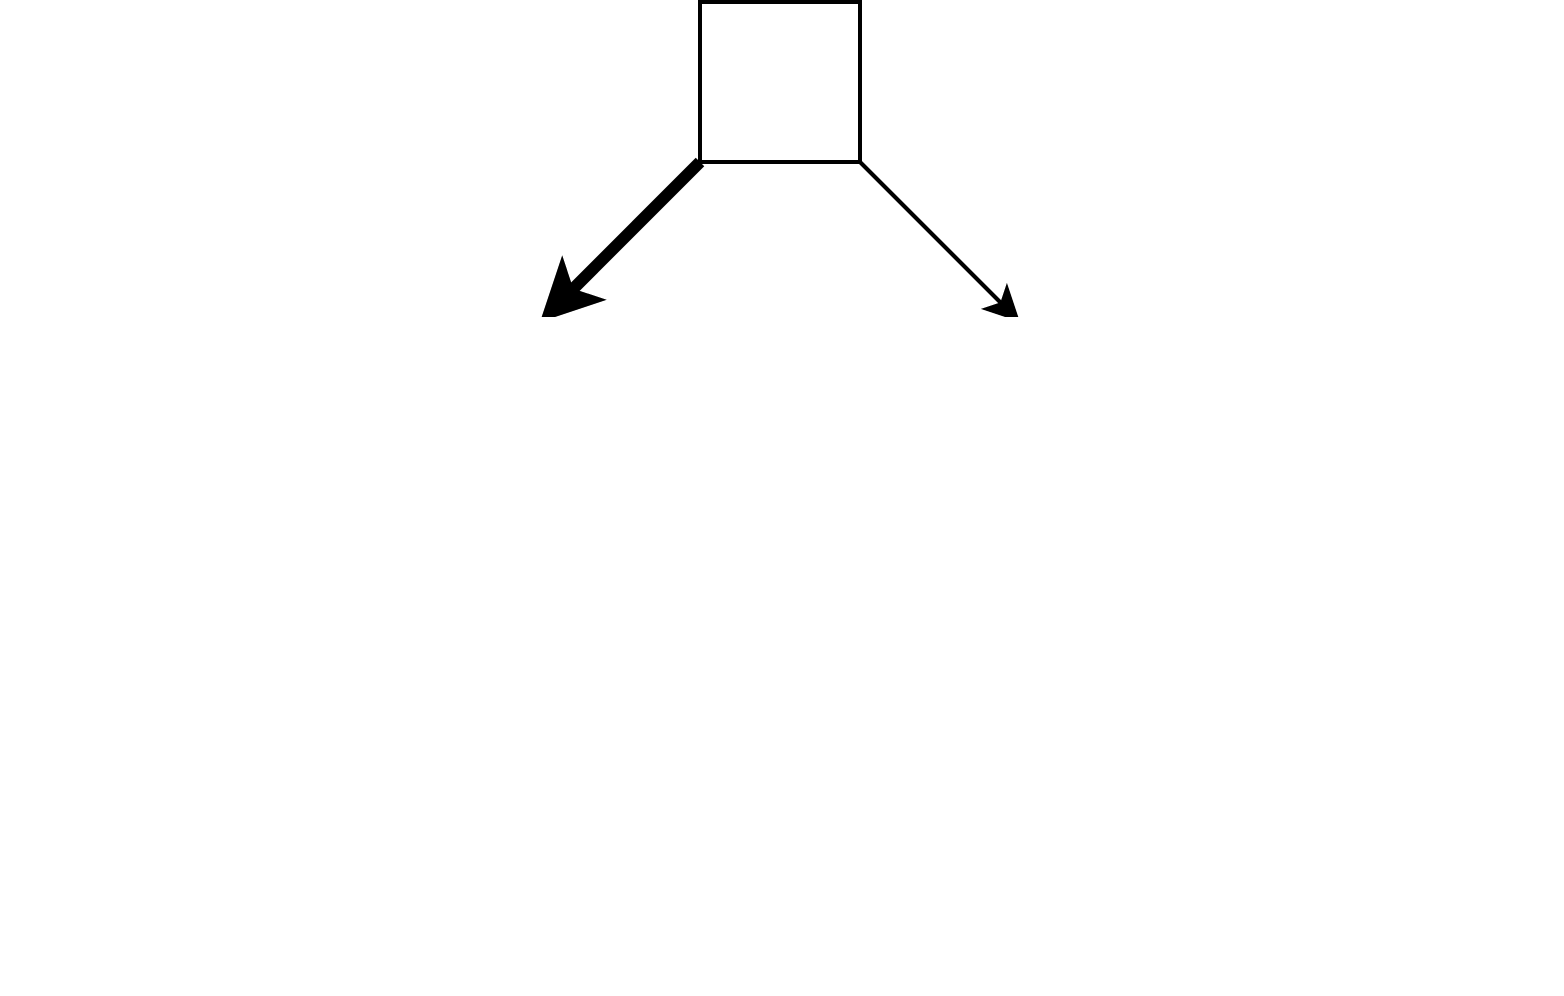
\includegraphics[scale=0.225]{tree_2}}
\only<3>{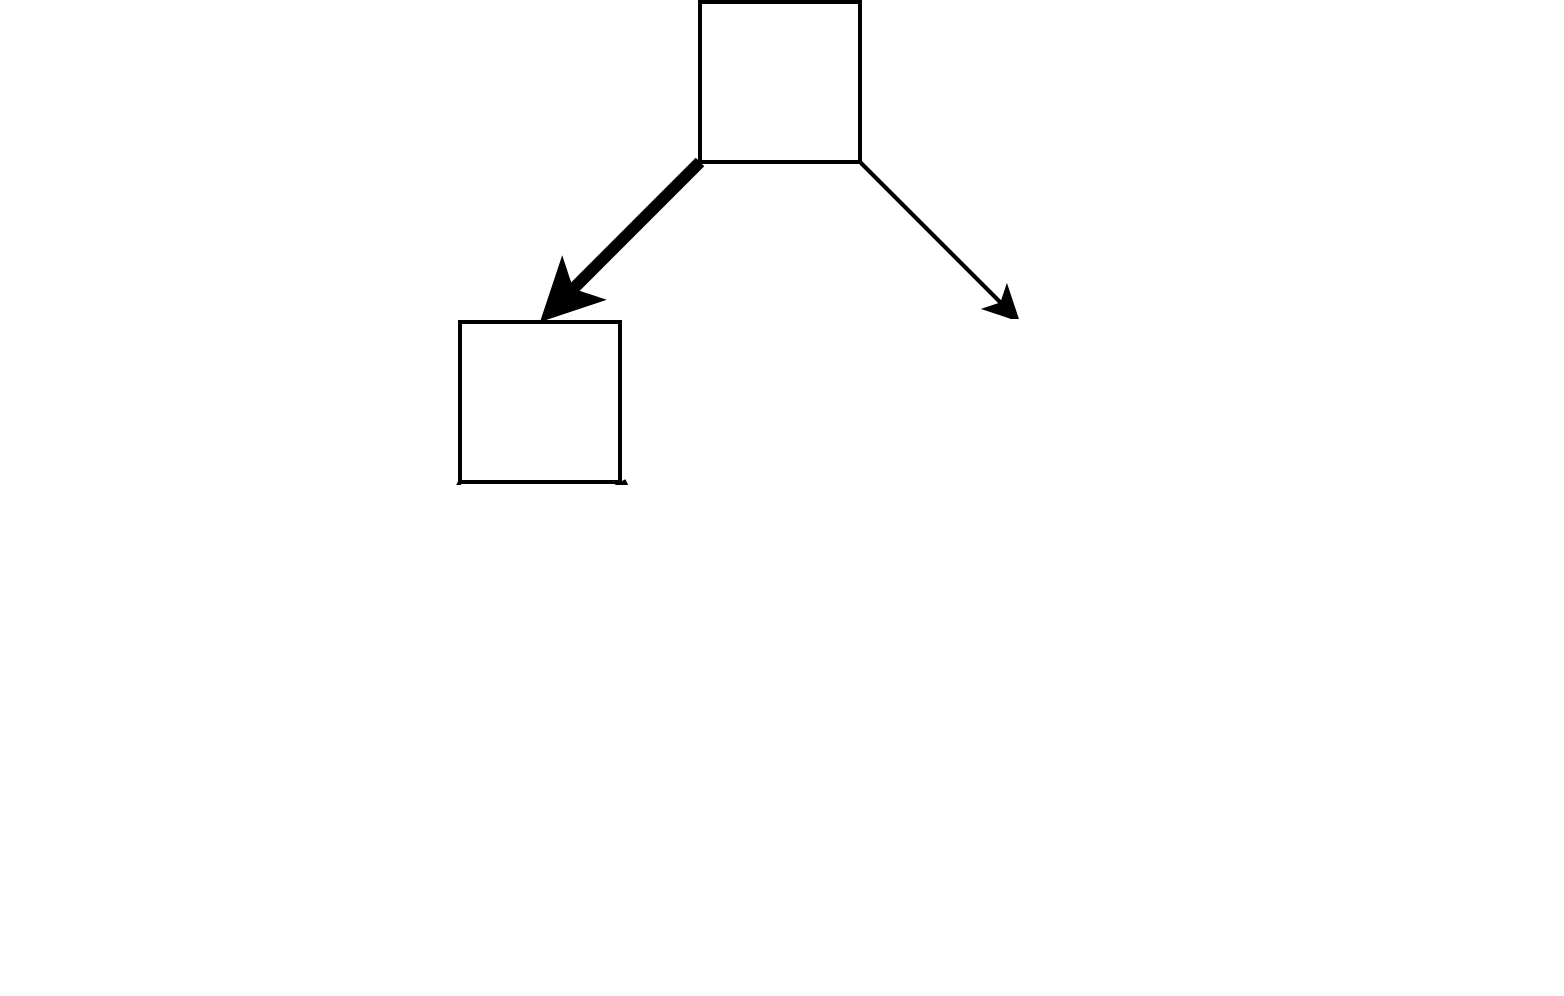
\includegraphics[scale=0.225]{tree_3}}
\only<4>{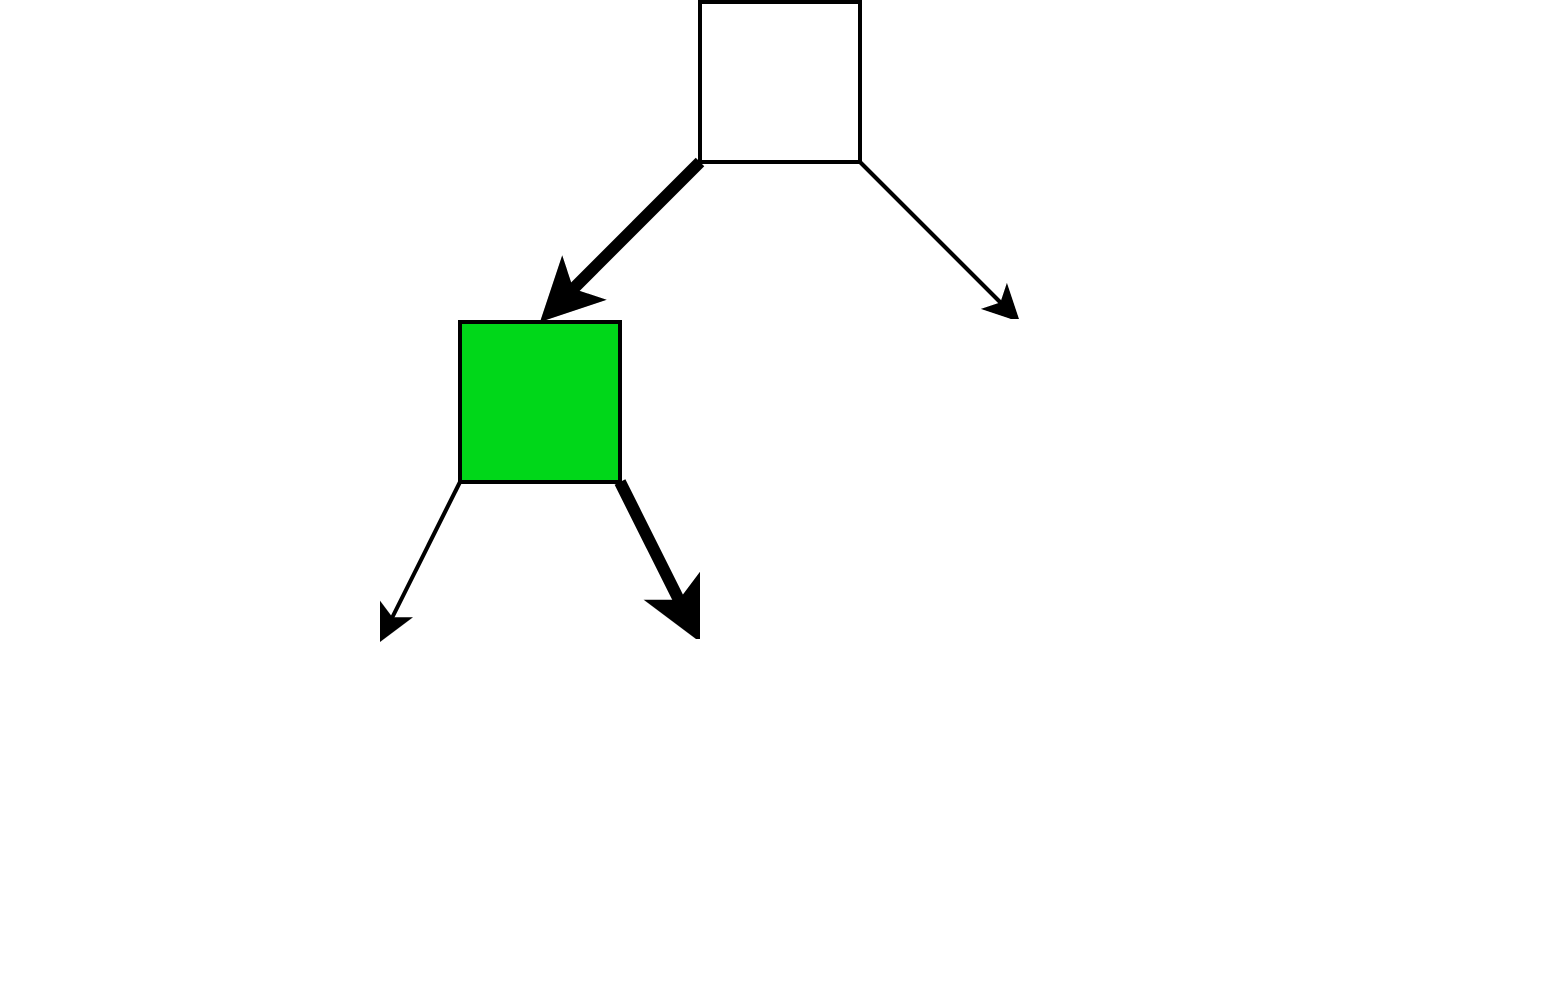
\includegraphics[scale=0.225]{tree_4}}
\only<5>{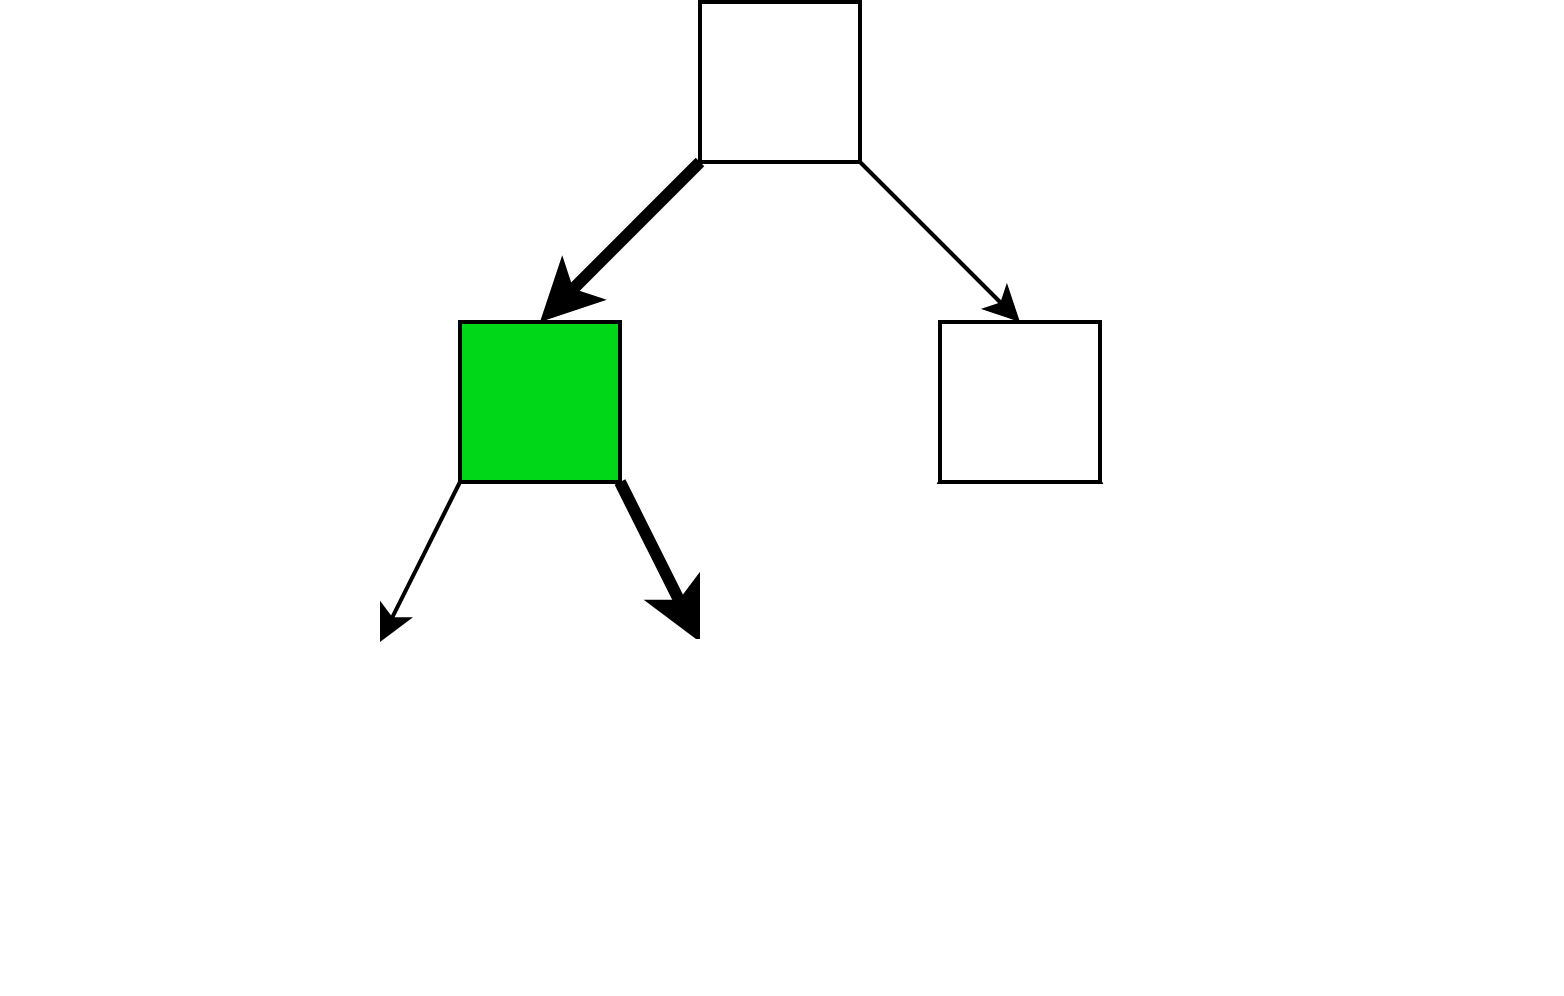
\includegraphics[scale=0.225]{tree_5}}
\only<6>{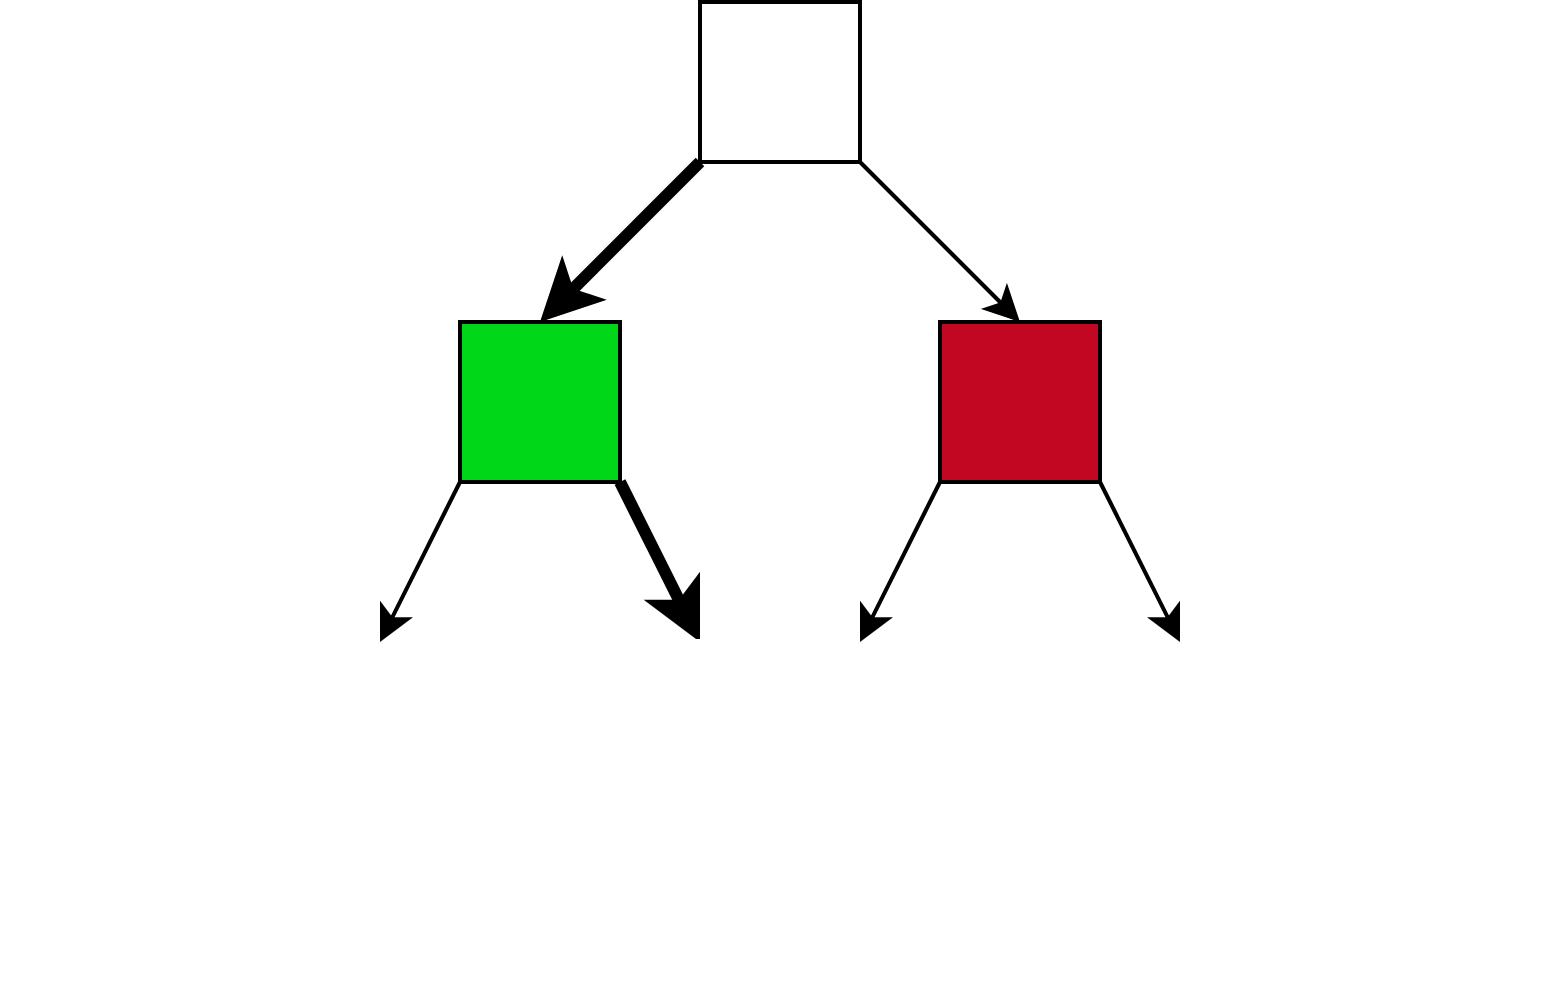
\includegraphics[scale=0.225]{tree_6}}
\only<7>{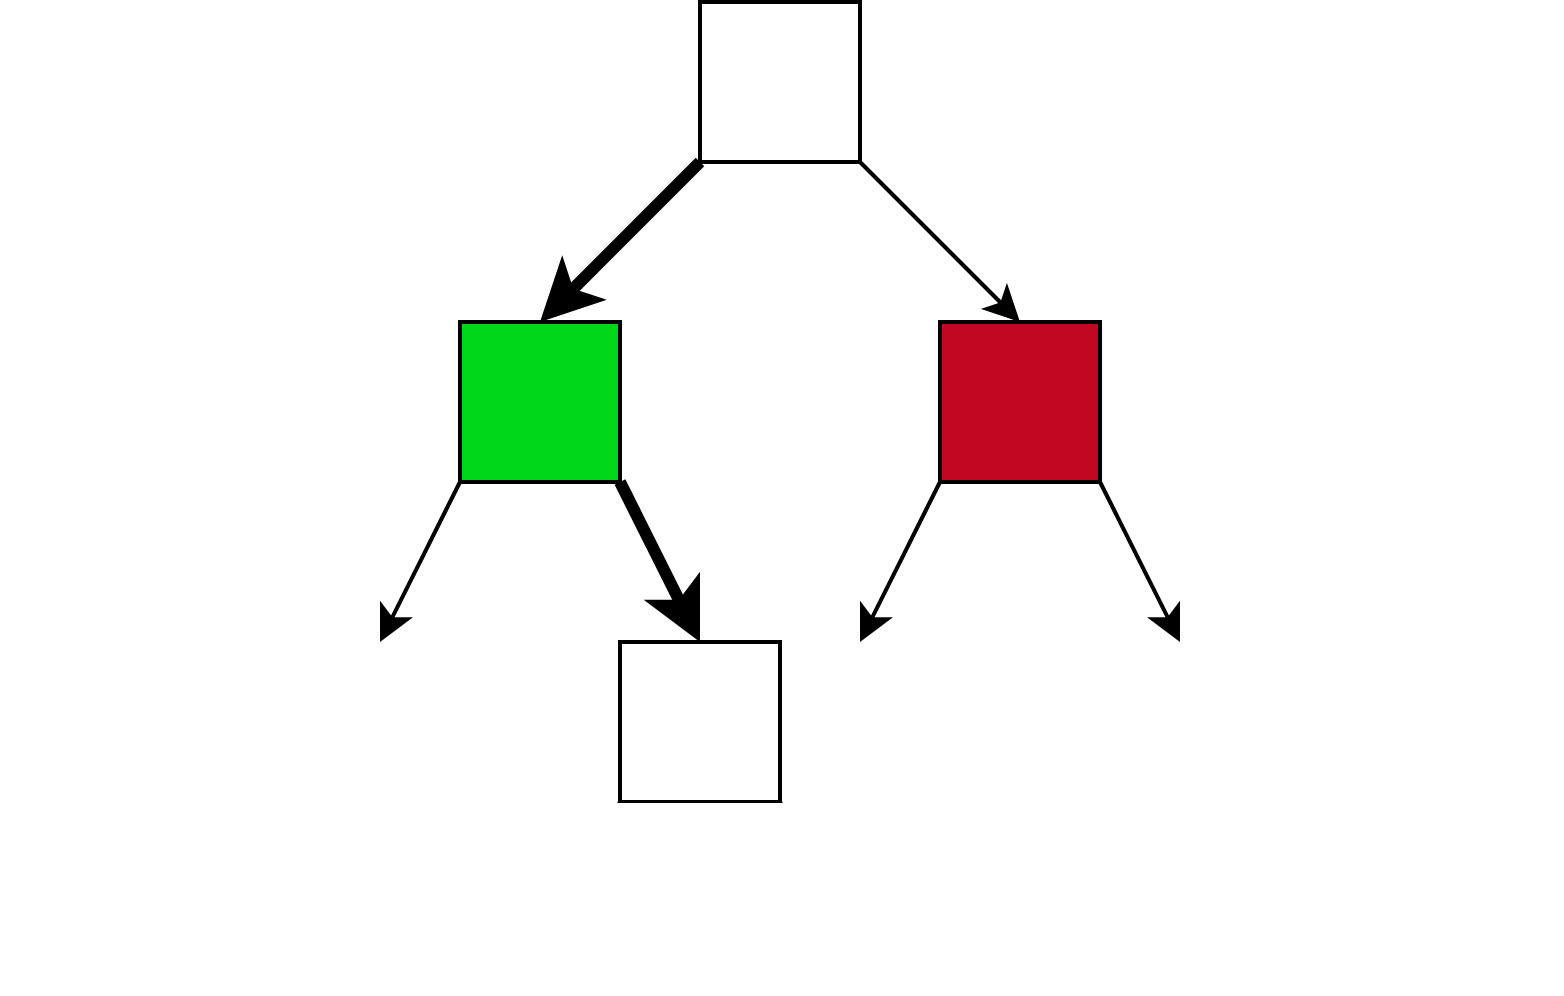
\includegraphics[scale=0.225]{tree_7}}
\only<8>{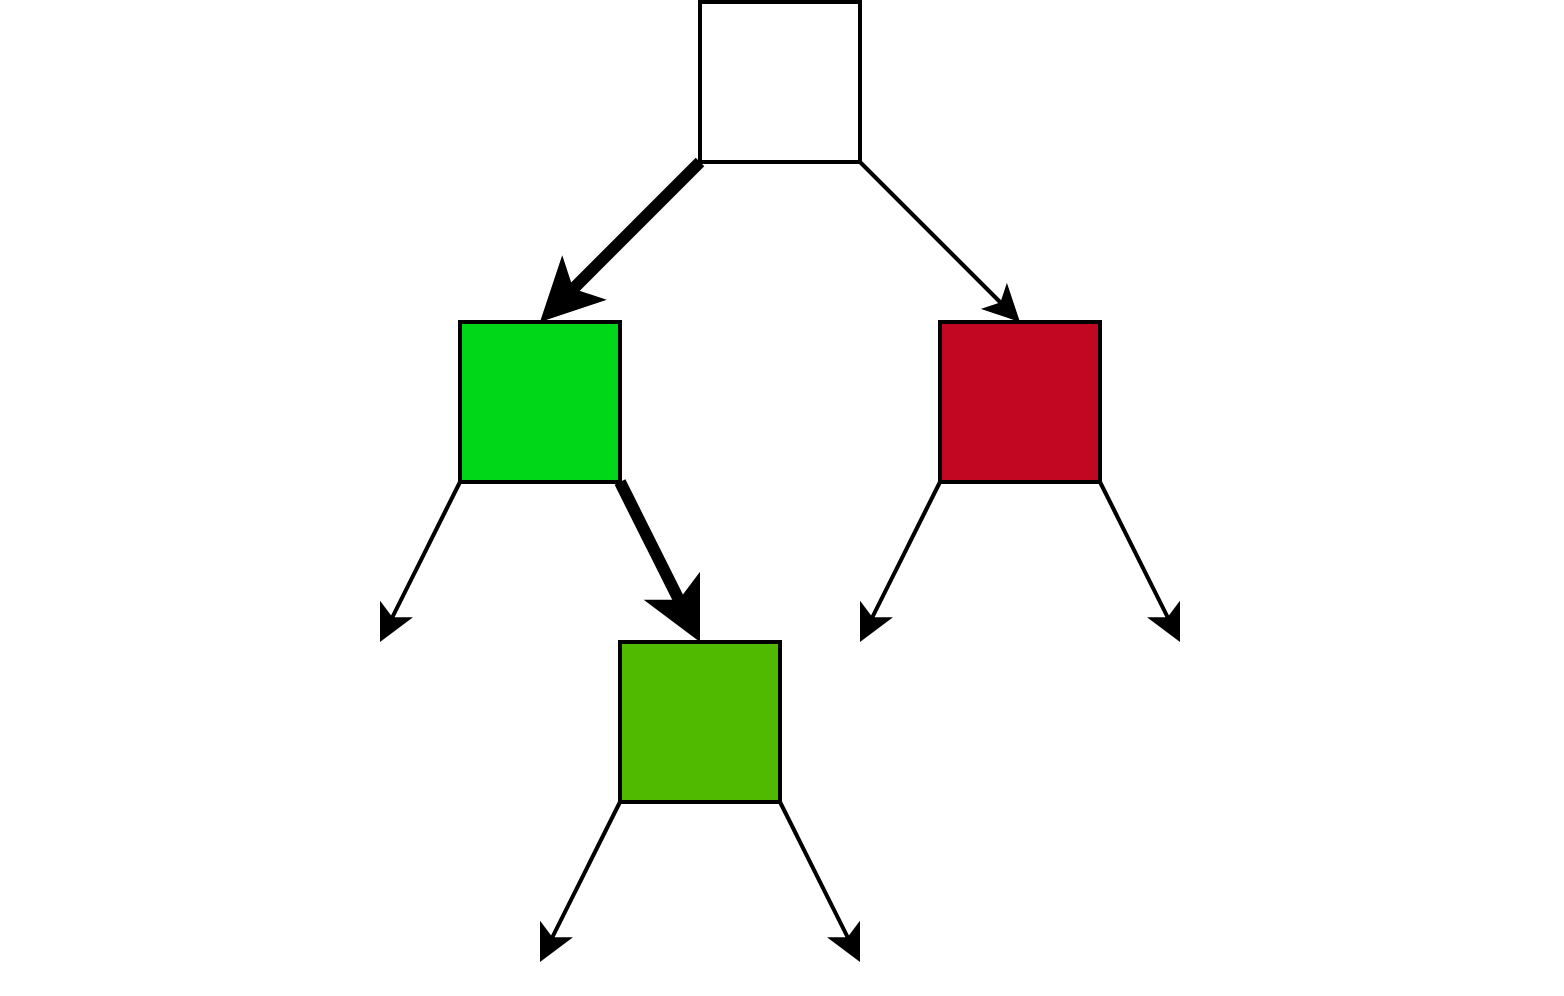
\includegraphics[scale=0.225]{tree_8}}


  
\end{frame}
\begin{frame}
 \frametitle{AlphaGo}
  


\begin{itemize}
  \item \pause Kernidee: Kombinere MCTS mit Deep Learning
  \item \pause Trainingsprozess involviert aber kein MCTS
  \item \pause Trainere mehrere Netzwerke
\begin{itemize}
  \item \pause Supervised auf Datensatz von besten Menschen: Schnell und Langsam
  \item \pause Verbessere das langsame Netz durch RL
  \item \pause Erzeuge Datensatz für Netzwerk zur Positionsevaluierung
  \item \pause Verwende erzeugte Netzwerke um mit MCTS zu spielen
\begin{itemize}
  \item \pause Das langsame RL-Netzwerk macht die Ersteinschätzung der Züge
  \item \pause Einschätzung der Spielposition: Netzwerk + Rollouts
\end{itemize}
\end{itemize}
\end{itemize}

  
\end{frame}
\begin{frame}
 \frametitle{AlphaZero}
  


\begin{itemize}
  \item \pause Drastische Vereinfachung von AlphaGo
  \item \pause Kernidee: Verwende MCTS bereits zur Trainingsphase
  \item \pause Verwendet nur ein Netzwerk: Positionsbewertung und Zugpolicy
  \item \pause Kein Bedarf für Datensatz von besten Menschen
\end{itemize}

  
\end{frame}
\begin{frame}
 \frametitle{AlphaZero: Trainingsablauf}
  


\begin{center}
\only<1>{
\includegraphics[scale=0.425]{a0_cycle_0}}
\only<2>{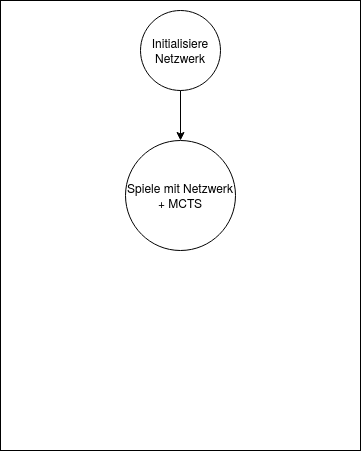
\includegraphics[scale=0.425]{a0_cycle_1}}
\only<3>{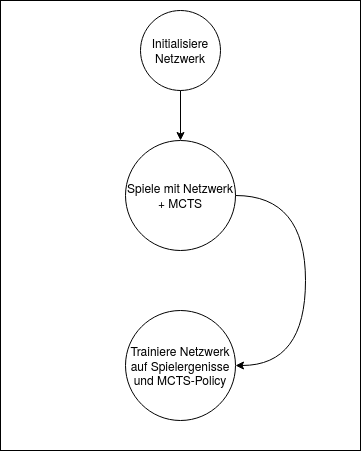
\includegraphics[scale=0.425]{a0_cycle_2}}
\only<4>{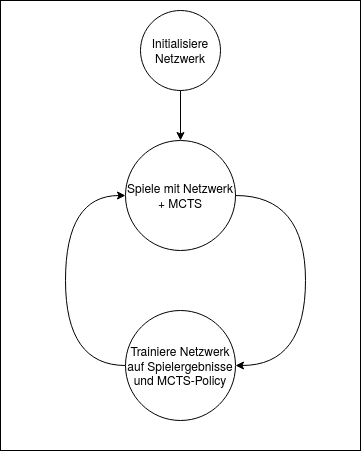
\includegraphics[scale=0.425]{a0_cycle_3}}
\end{center}

  
\end{frame}

\subsection{Baselines}



\begin{frame}
 \frametitle{Aufbau der Experimente}
  


\only<1>{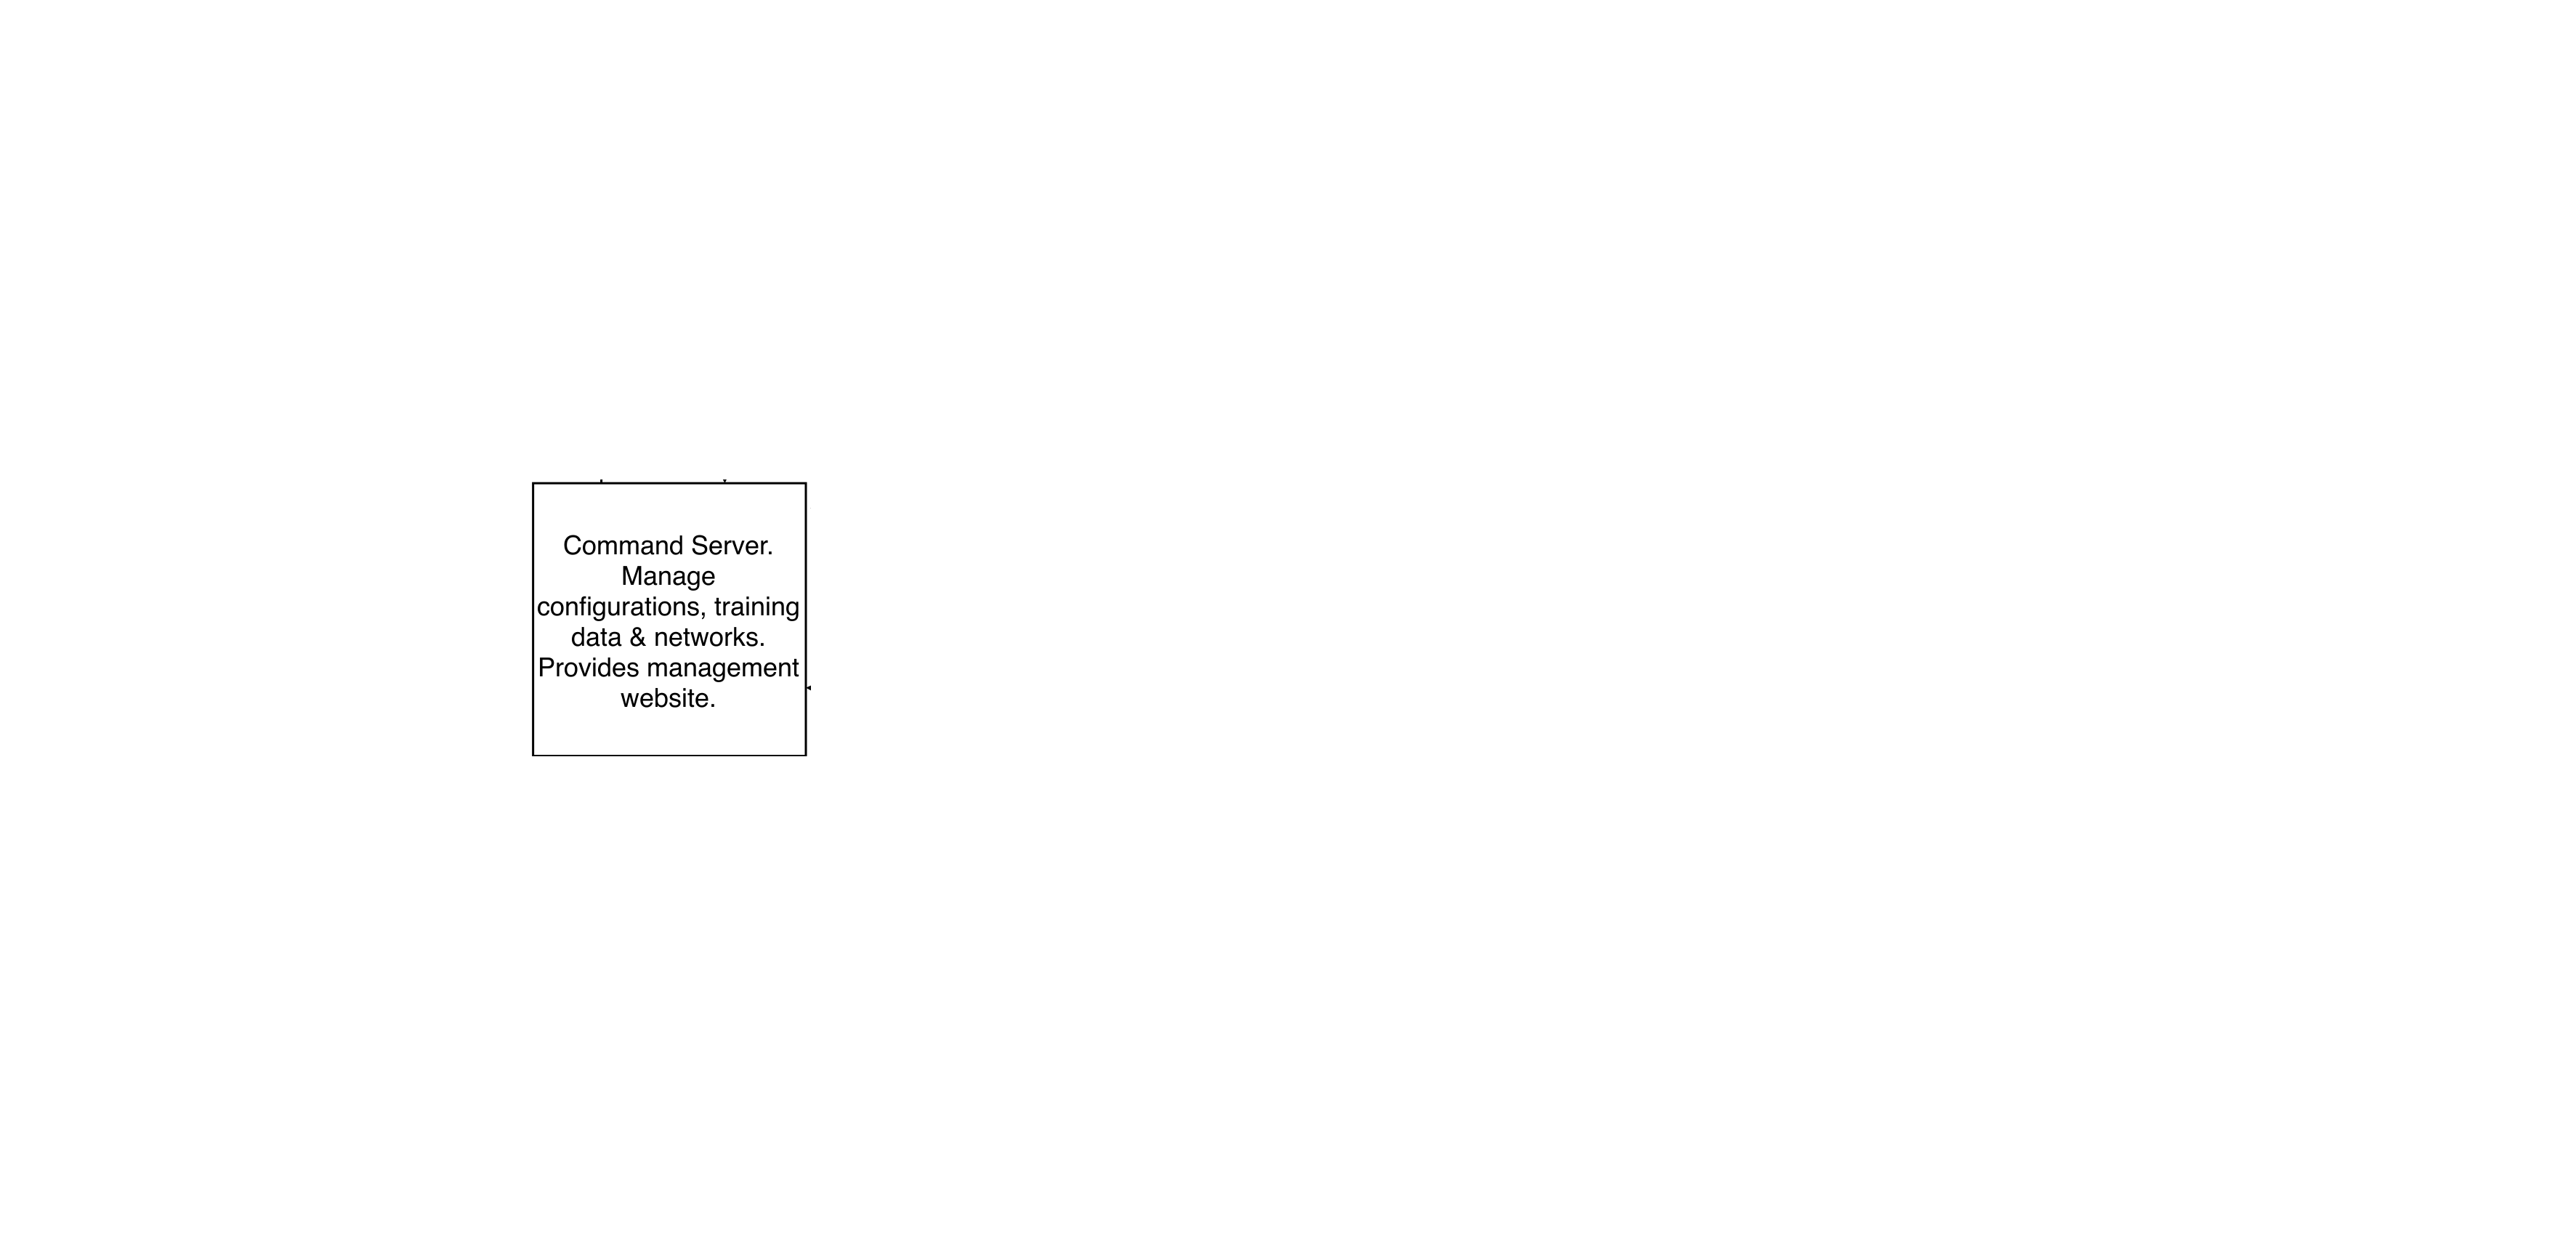
\includegraphics[scale=0.425]{framework_0}}
\only<2>{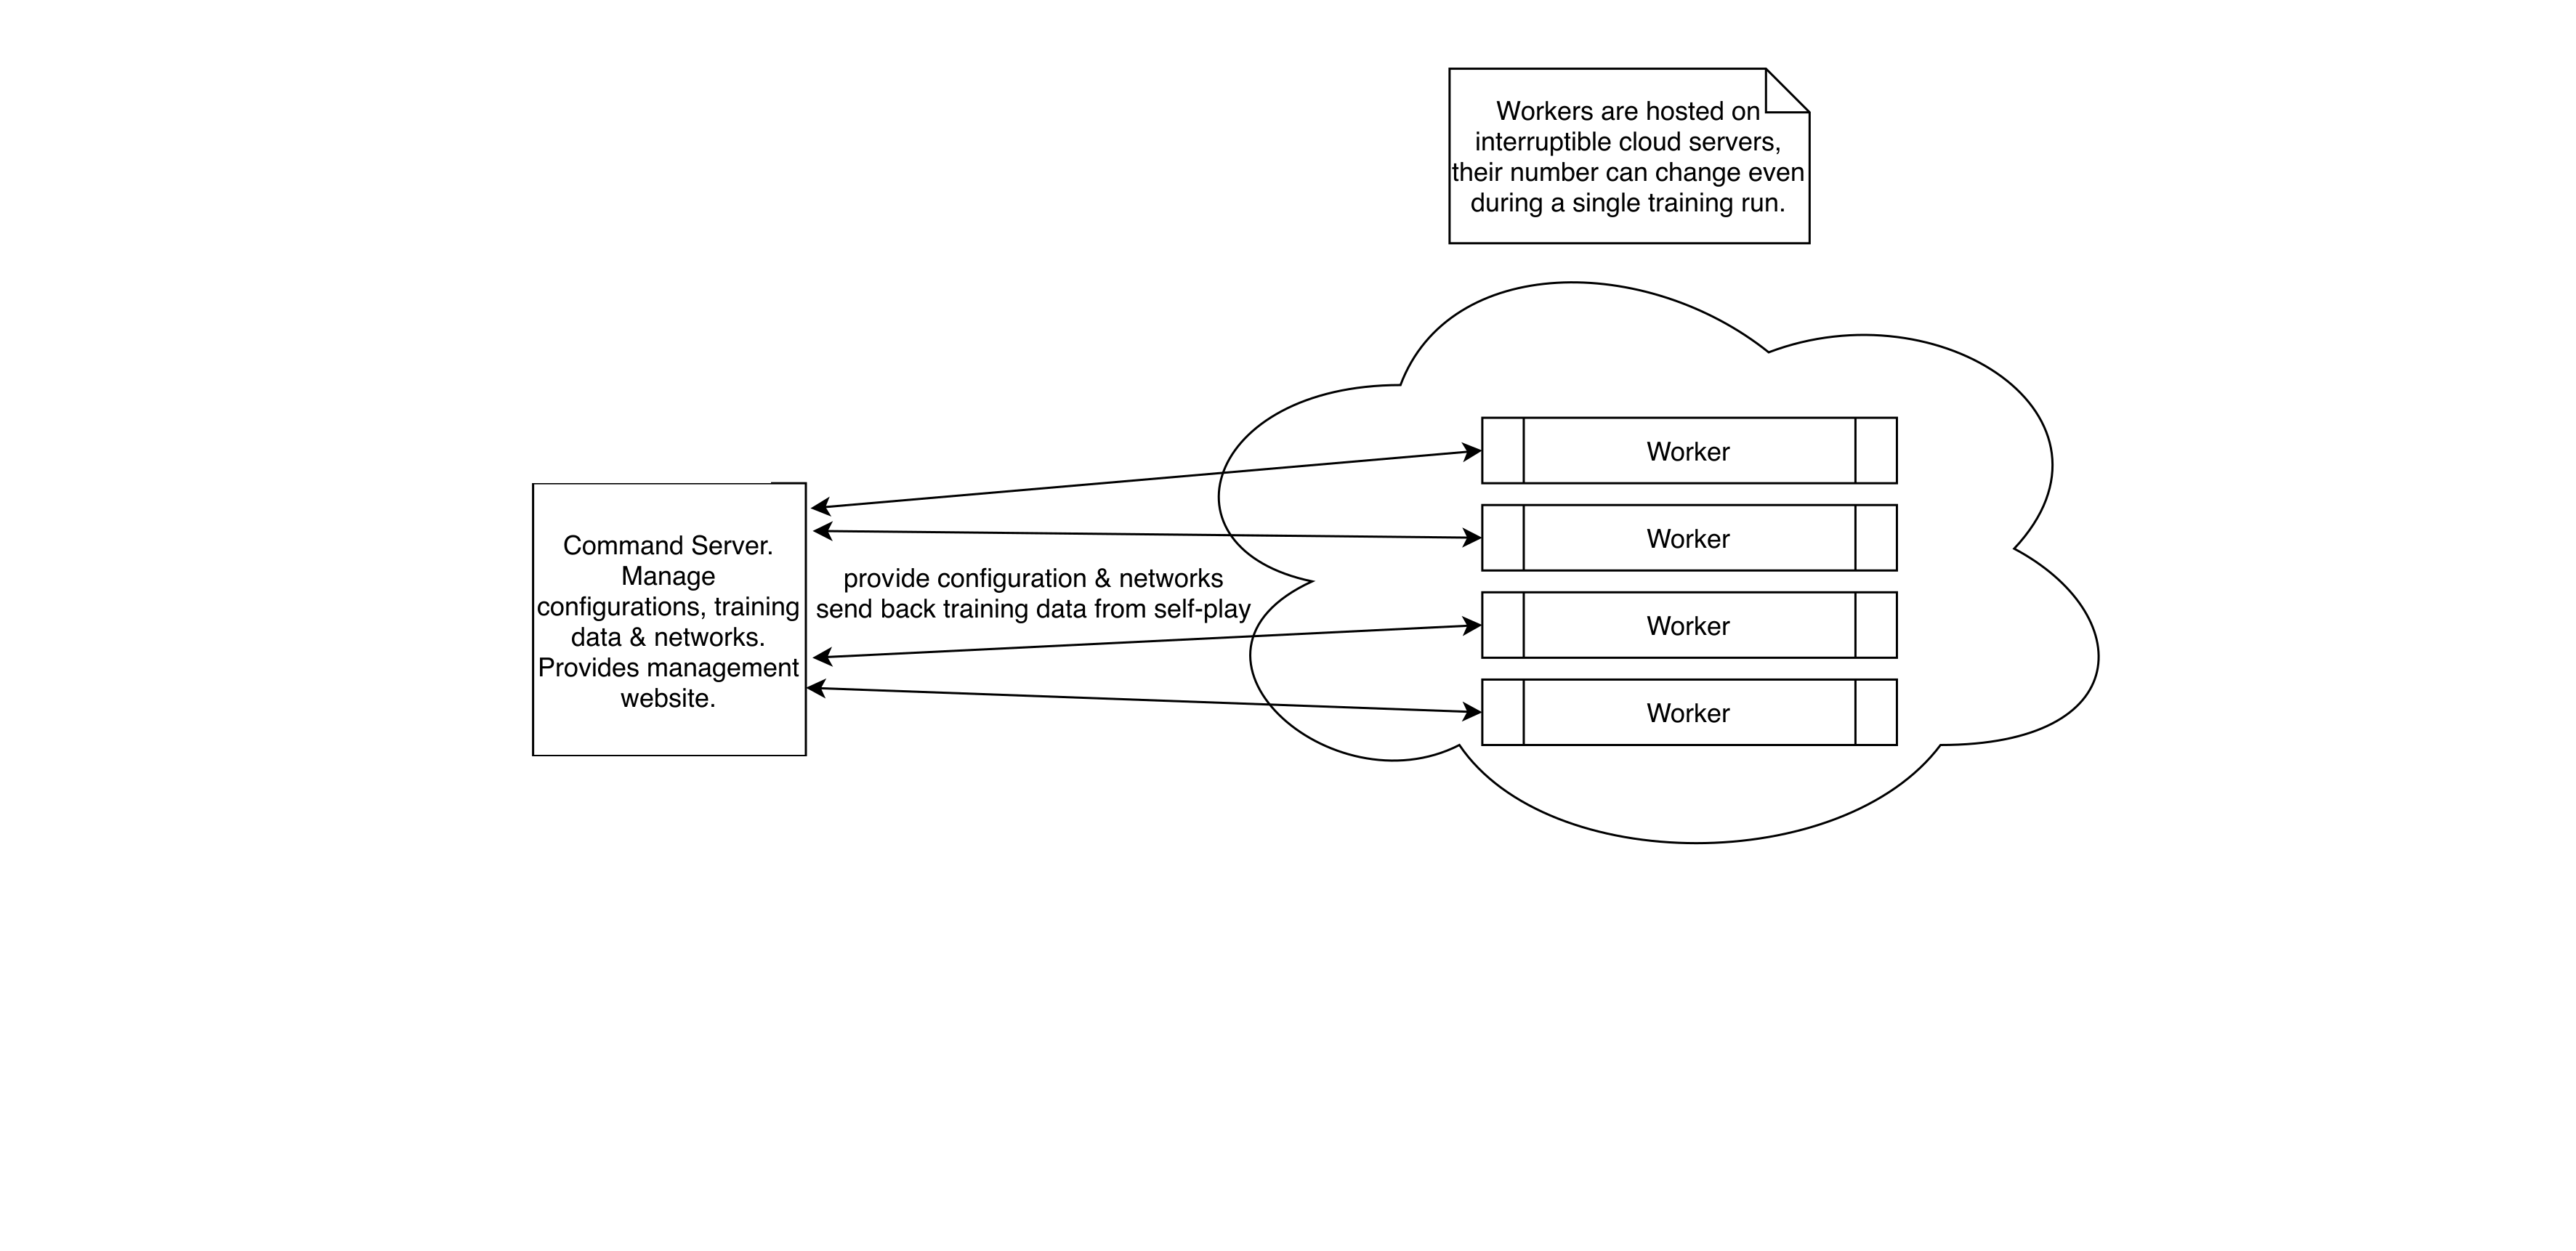
\includegraphics[scale=0.425]{framework_1}}
\only<3>{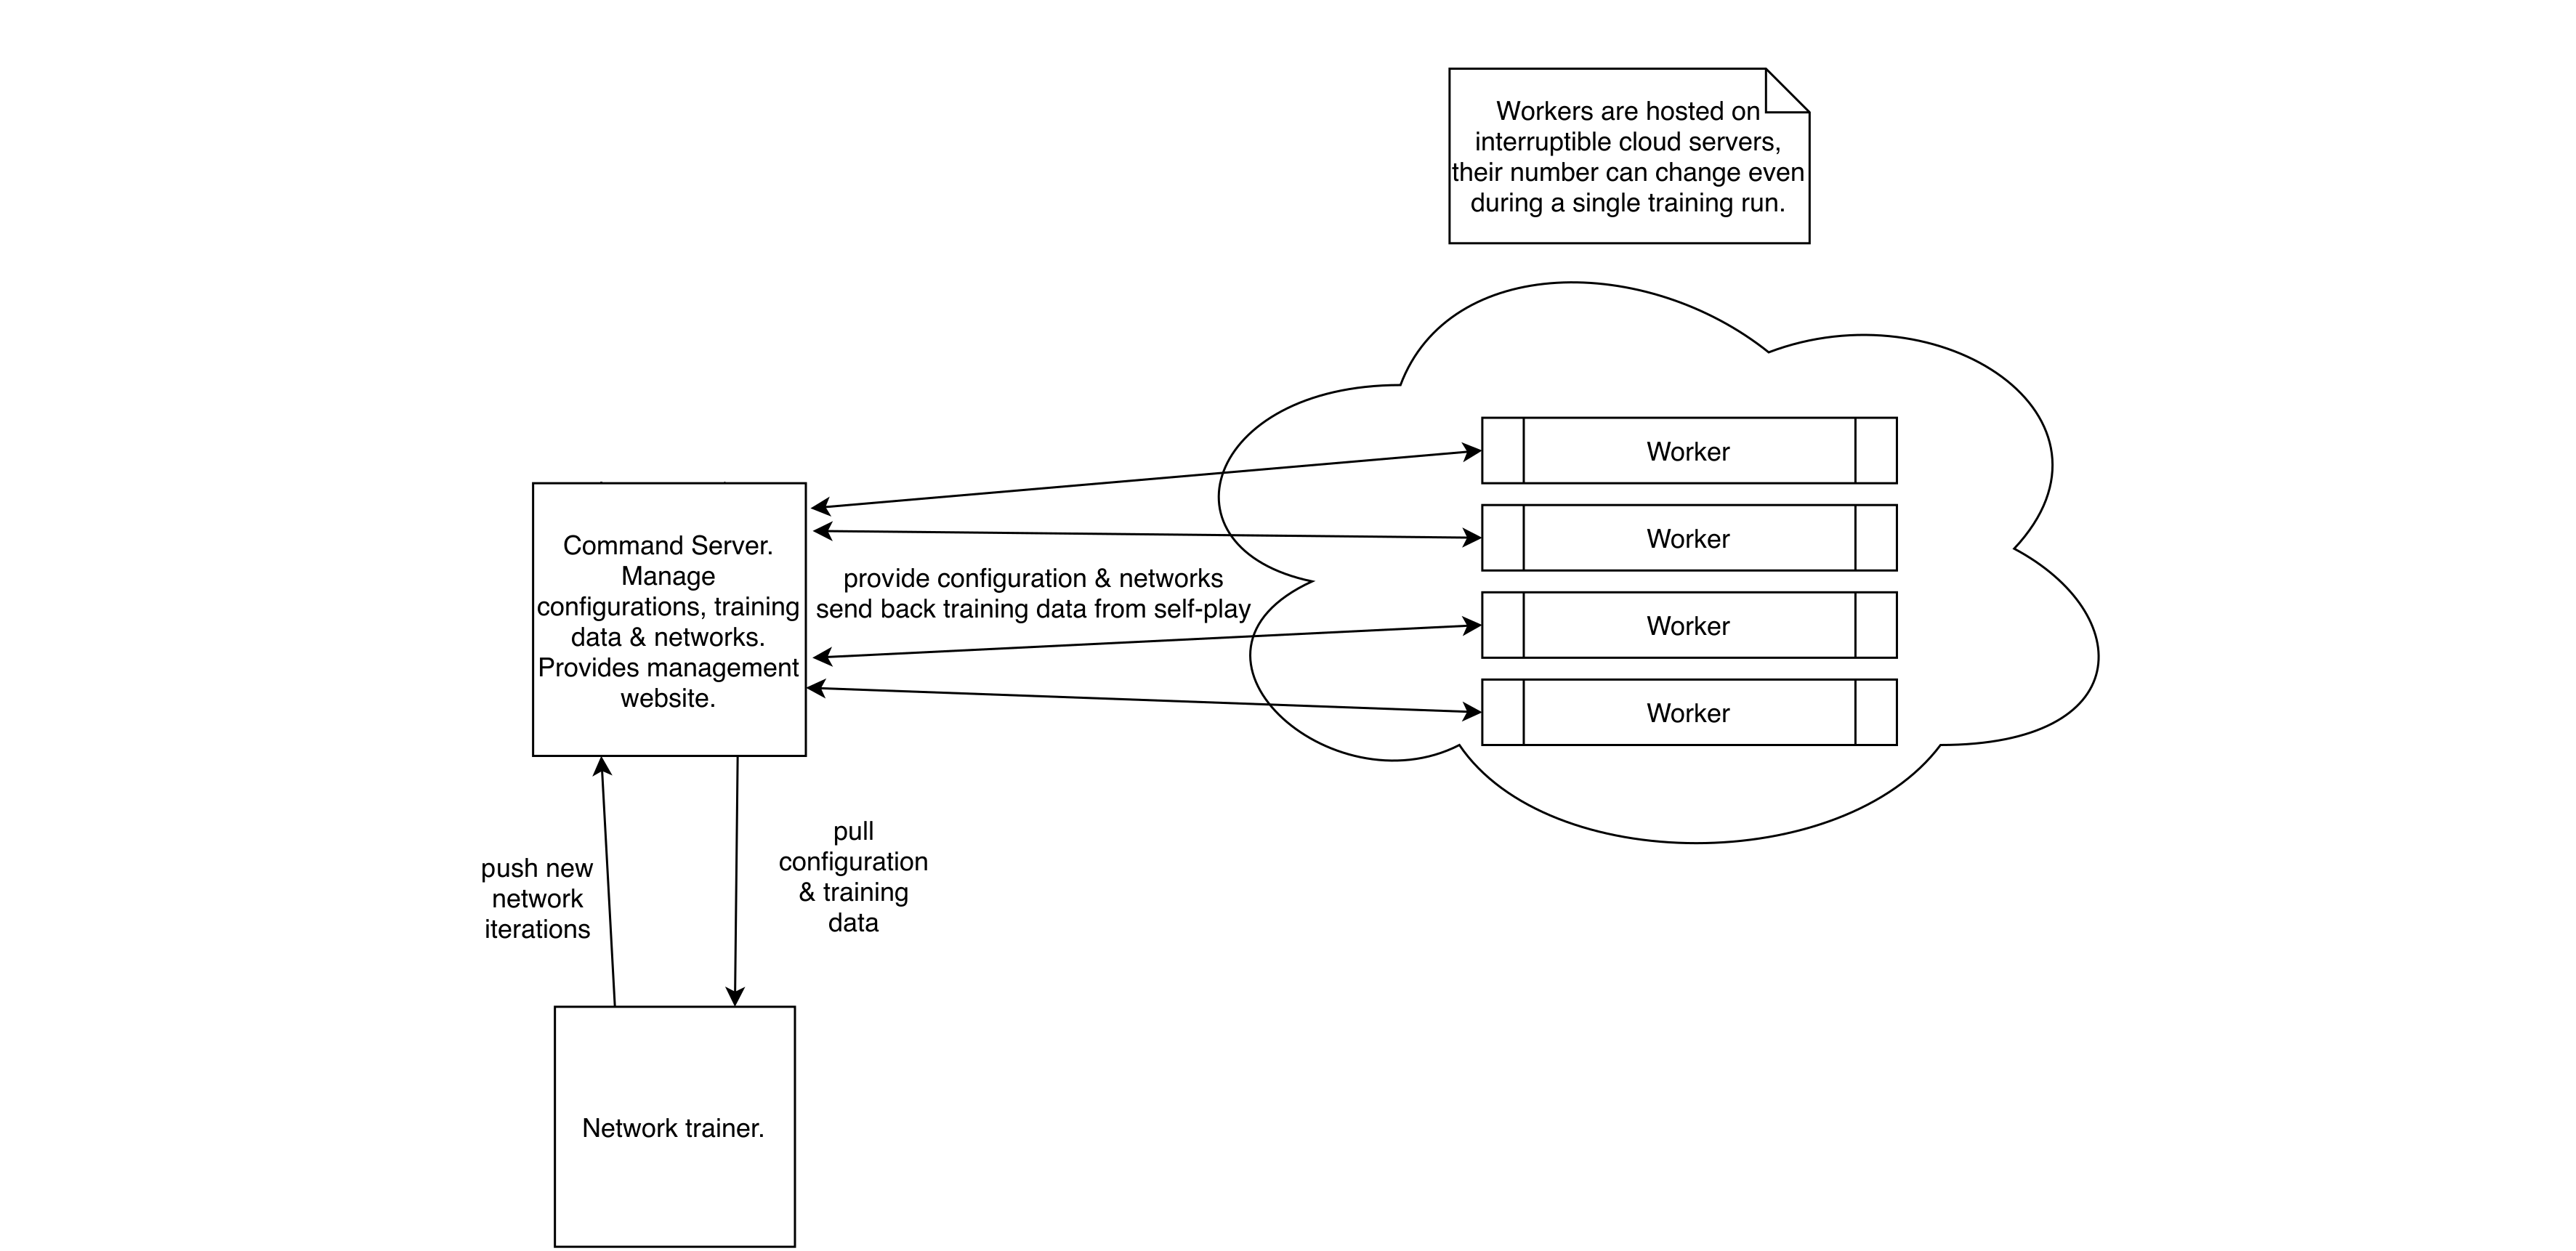
\includegraphics[scale=0.425]{framework_2}}
\only<4>{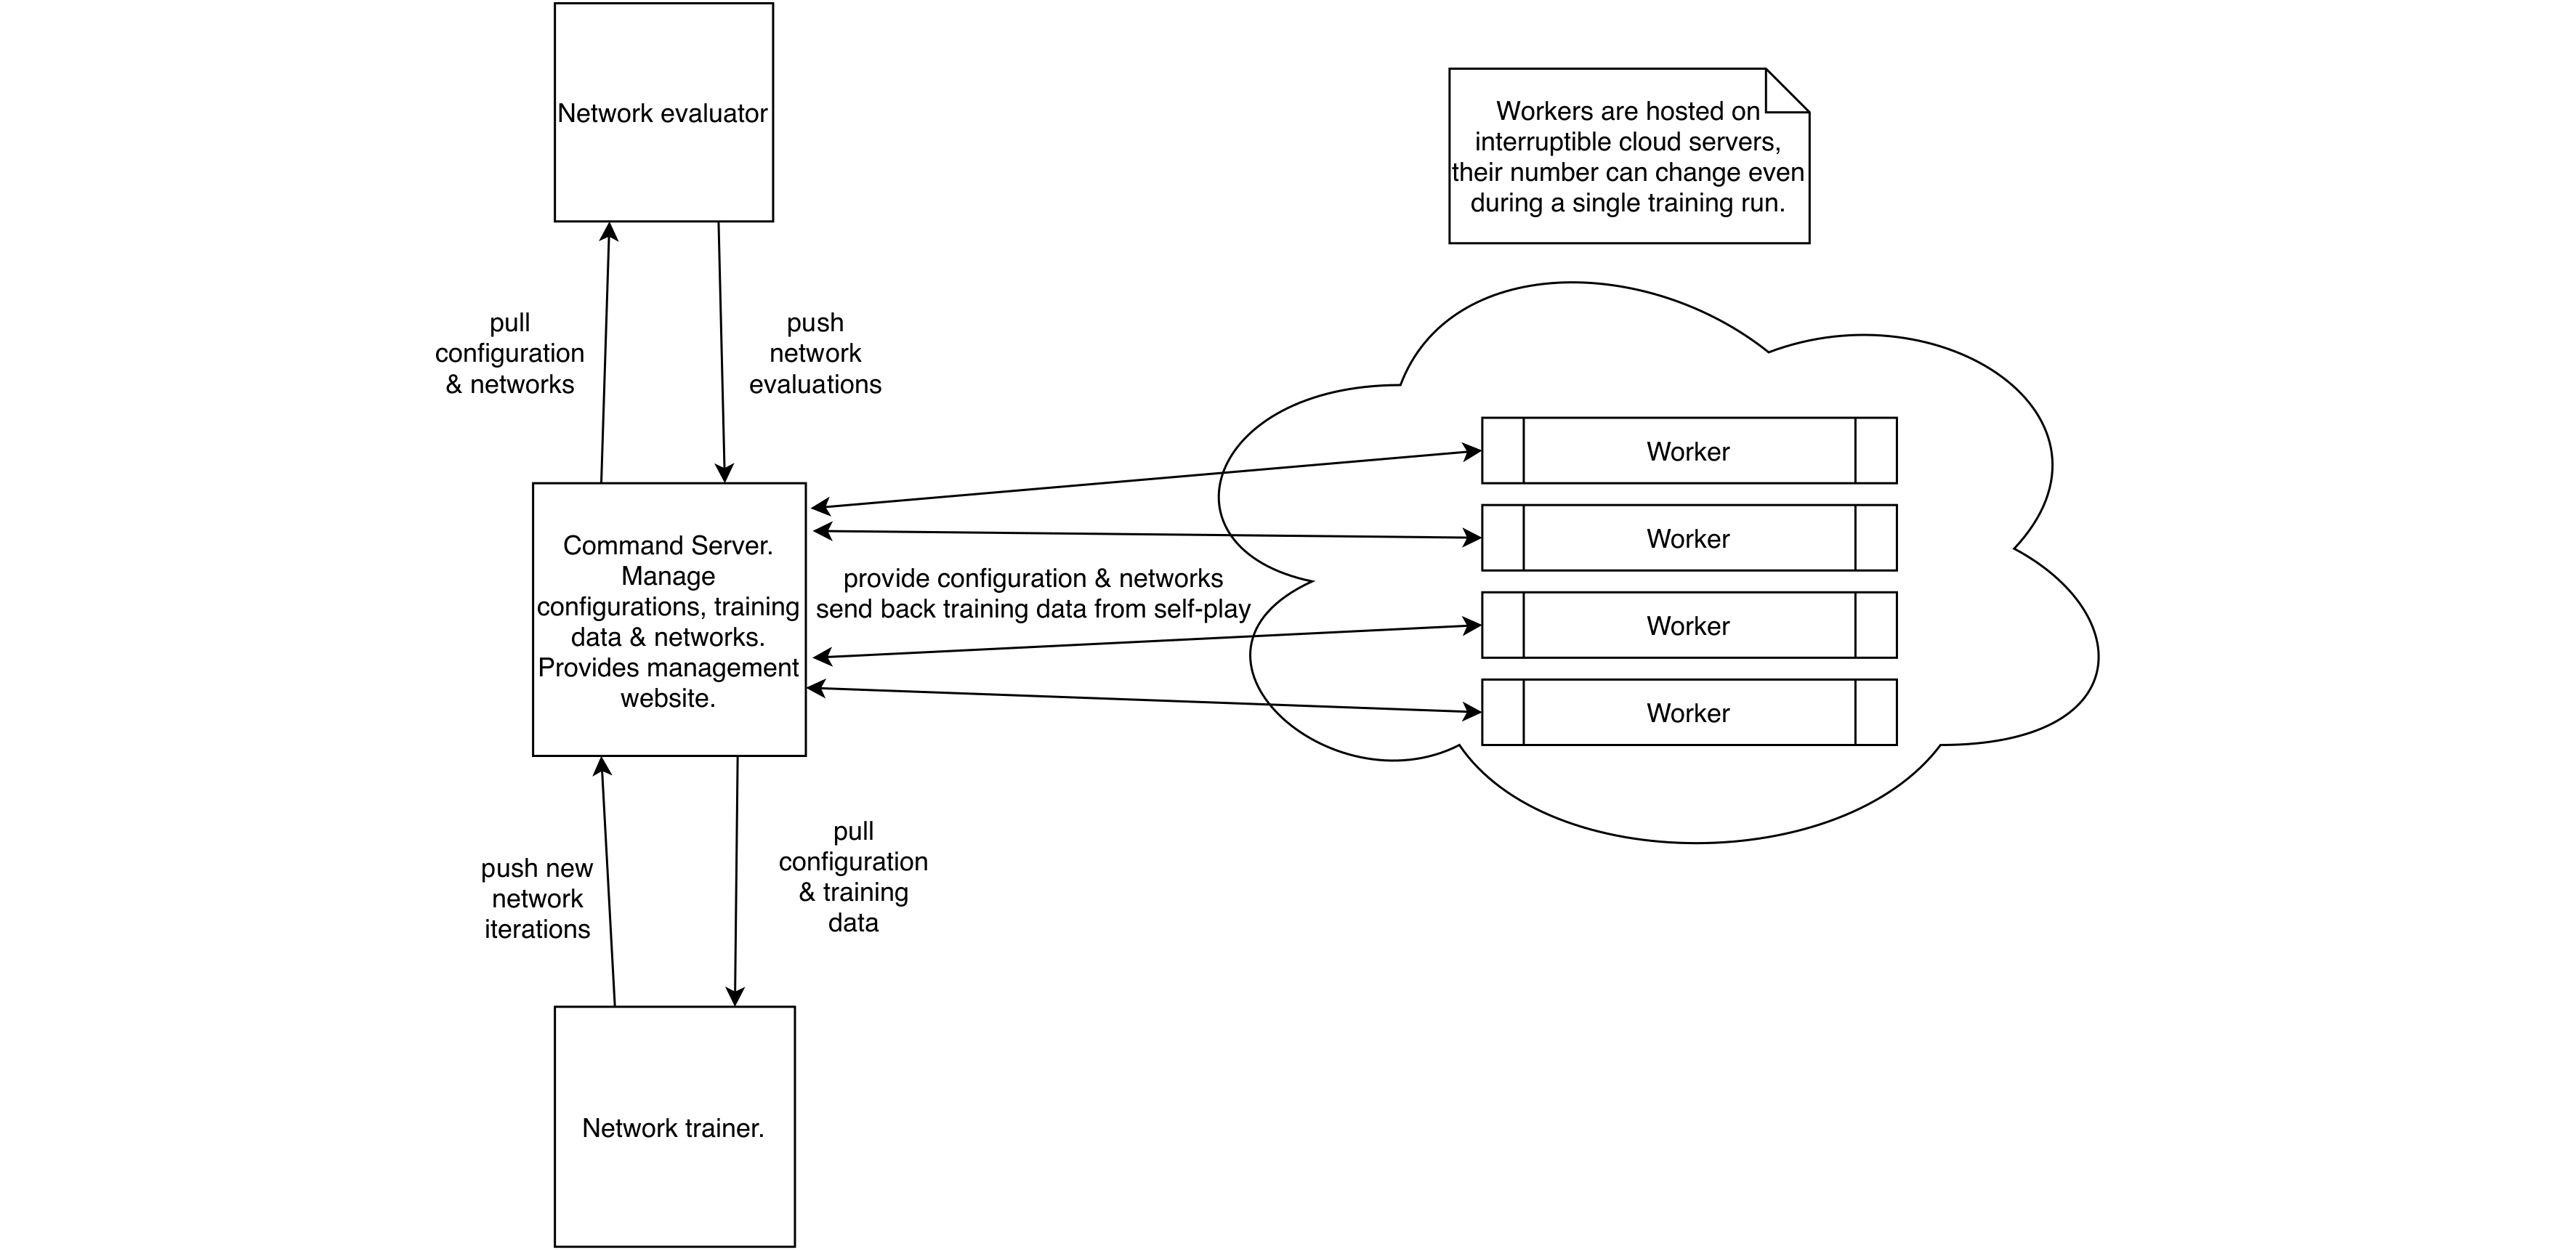
\includegraphics[scale=0.425]{framework_3}}

  
\end{frame}
\begin{frame}
 \frametitle{Hyperparametersuche}
  


\begin{itemize}
  \item \pause Optimiere wichtige Hyperparameter für Vier gewinnt
  \item \pause Bayesian Optimization Package verwendet
  \item \pause Fitnessfunktion: Trainiere über 2 Stunden, messe Accuracy
  \item \pause 65 Steps, Laufzeit ca. eine Woche
\end{itemize}
\only<6>{\center 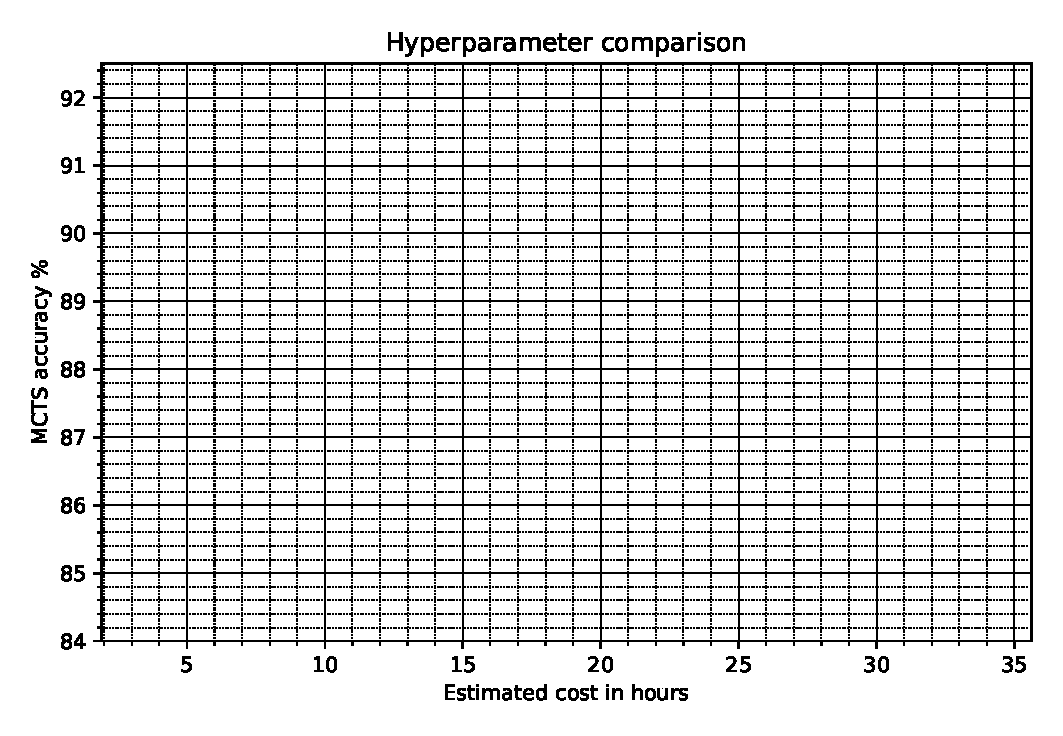
\includegraphics[scale=0.425]{hyper_compare0}}
\only<7>{\center 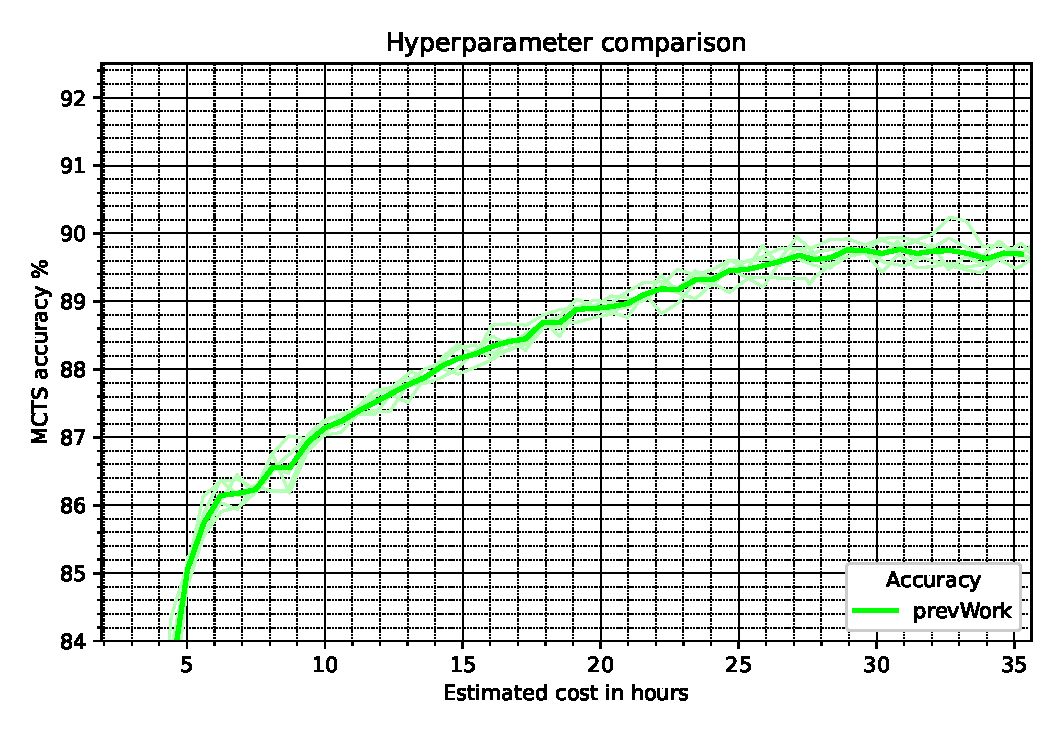
\includegraphics[scale=0.425]{hyper_compare1}}
\only<8>{\center 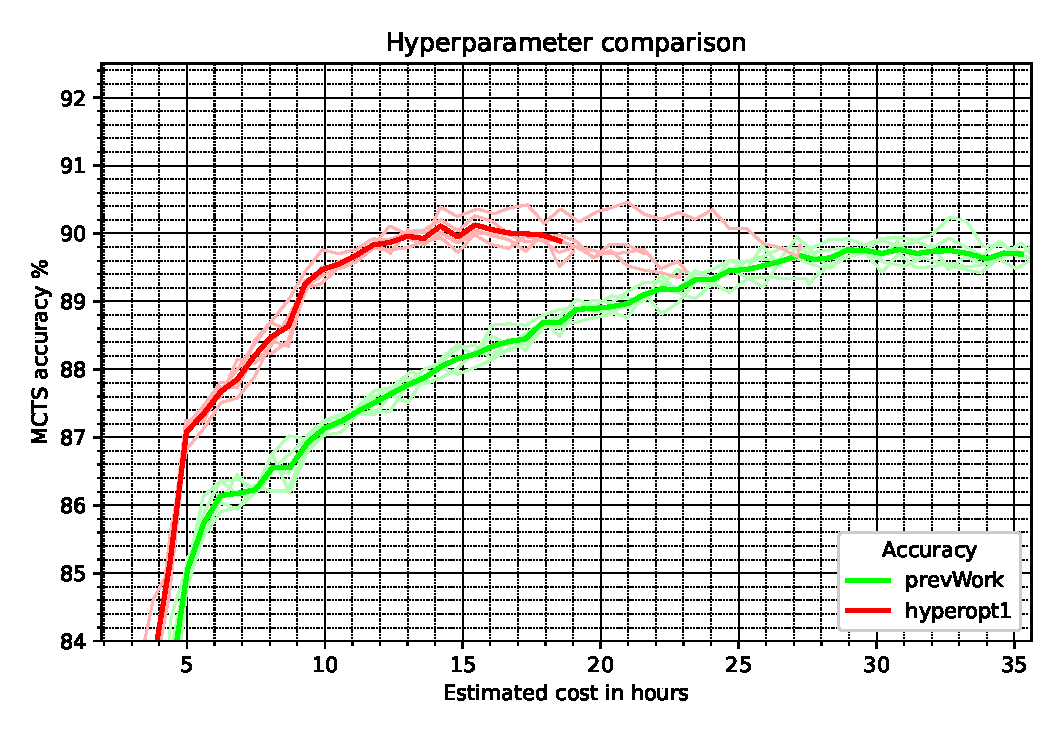
\includegraphics[scale=0.425]{hyper_compare2}}
\only<9>{\center 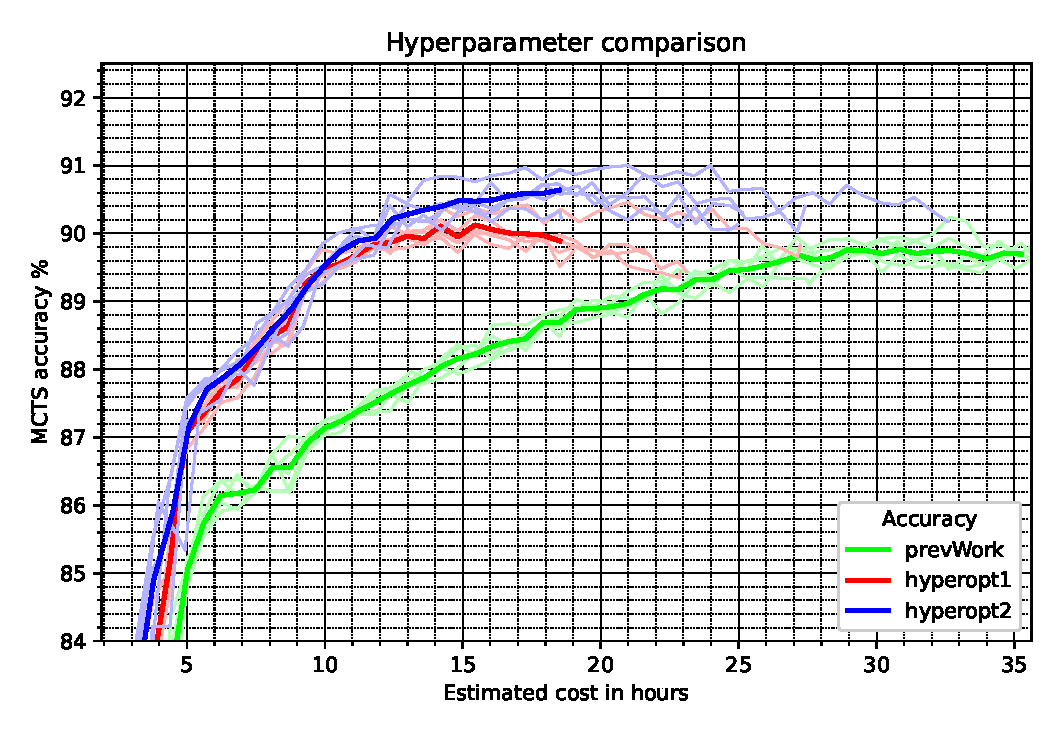
\includegraphics[scale=0.425]{hyper_compare}}



  
\end{frame}
\begin{frame}
 \frametitle{Extended baseline}
  


\begin{itemize}
  \item \pause Erweitere die Baselineimplementierung mit Verbesserungen anderer Arbeiten
\begin{itemize}
  \item \pause Deduplikation
  \item \pause Cyclic learning rate
  \item \pause Verbessertes Trainingswindow
  \item \pause Playout Caps
  \item \pause Vorhersage des nächsten Zuges des Gegners
  \item \pause Verbesserung des Netzwerks
\end{itemize}
\end{itemize}

\begin{itemize}
  \item \pause Alle außer Playout Caps zeigten eine tendenzielle Verbesserung
  \item \pause Kombiniert ist die Verbesserung sehr erheblich.
\end{itemize}

  
\end{frame}
\begin{frame}
 \frametitle{Extended baseline Ergebnisse}
  


\only<1>{\center 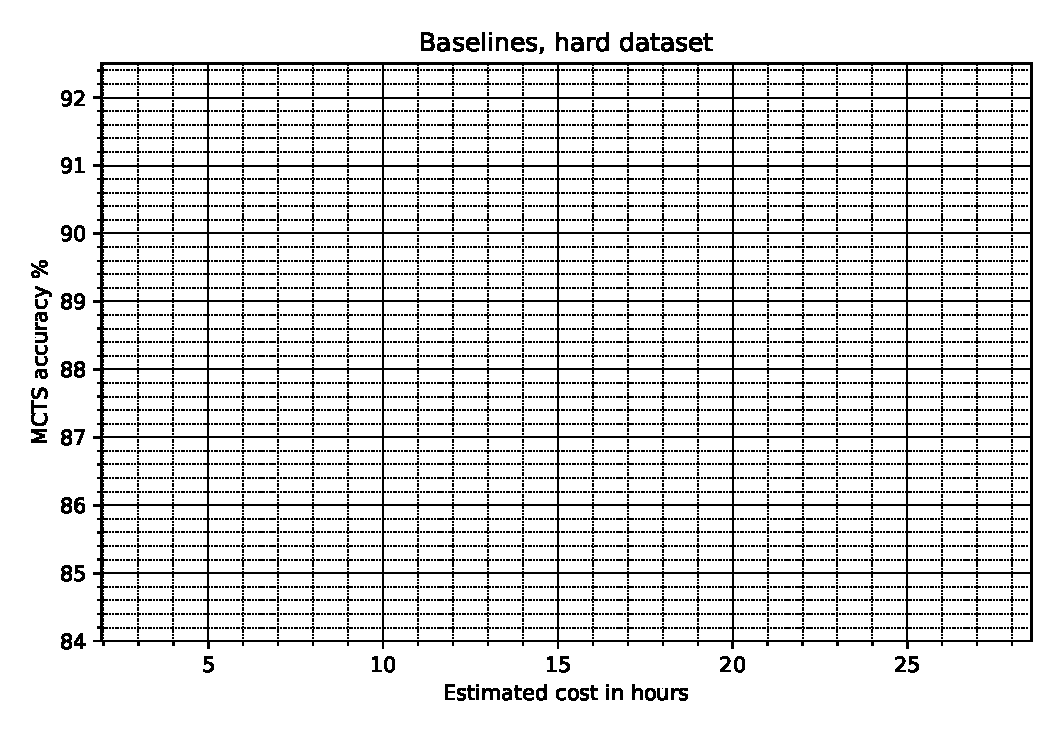
\includegraphics[scale=0.625]{baseline_ex0}}
\only<2>{\center 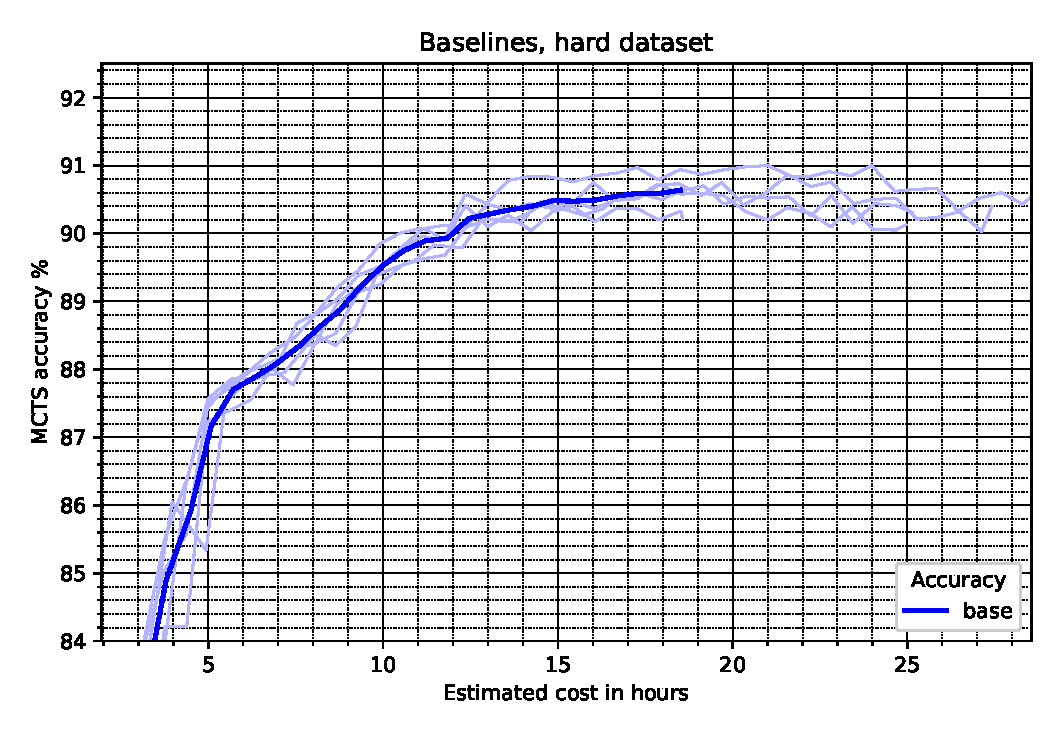
\includegraphics[scale=0.625]{baseline_ex1}}
\only<3>{\center 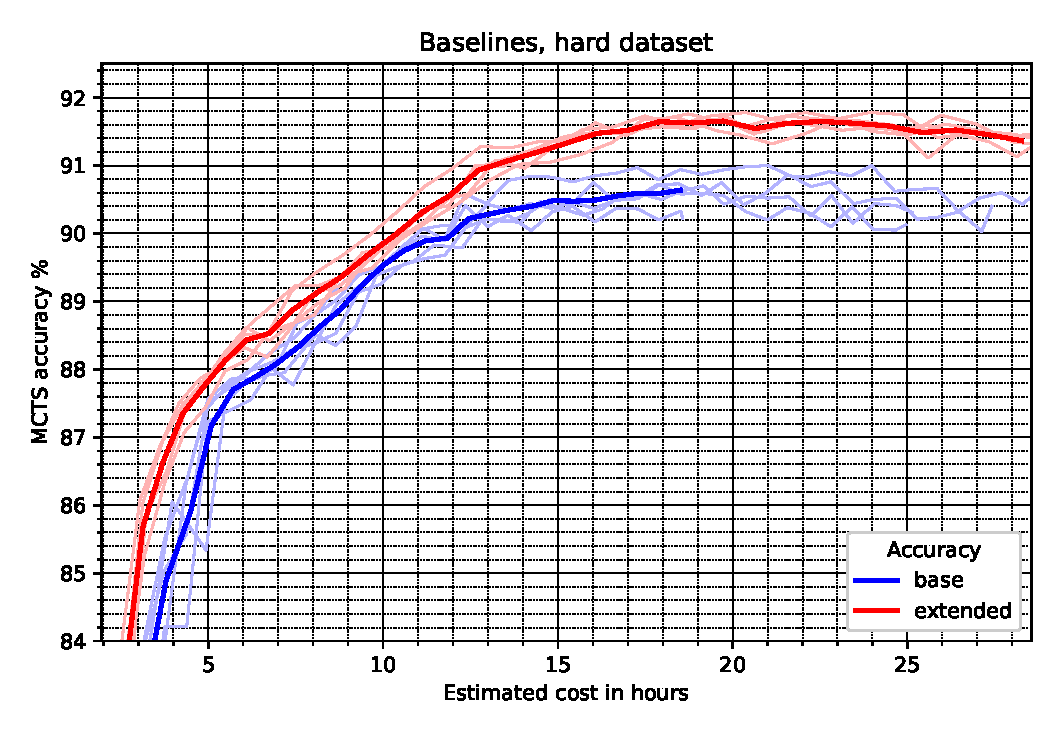
\includegraphics[scale=0.625]{baseline_ex}}

  
\end{frame}

\section{Untersuchte neue Ideen}




\subsection{Evolutionary Self-play}



\begin{frame}
 \frametitle{Implementierung: Evolutionary Self-play}
  


\begin{itemize}
  \item \pause Verwende die Self-play-phase zur Evolution von Hyperparametern
  \item \pause Beschränkt auf Hyperparameter, welche sich leicht ändern lassen
  \item \pause Implementiert als eine Liga von Spielern.
  \item \pause Ein Spieler ist ein Hyperparameterset
  \item \pause Bewerte Spieler mit Elo
  \item \pause Verwende Gaussian Mutation um die besten Spieler zu mutieren
\end{itemize}

\begin{itemize}
  \item \pause Zwei Arten von Hyperparametern untersucht
\begin{itemize}
  \item \pause Verwendung von Kullback-Leibler divergence um "Denkzeit" zu wählen.
  \item \pause MCTS Parameter: cpuct, fpu, drawValue
\end{itemize}
\end{itemize}

  
\end{frame}
\begin{frame}
 \frametitle{Erste Ergebnisse}
  


\only<1>{\center 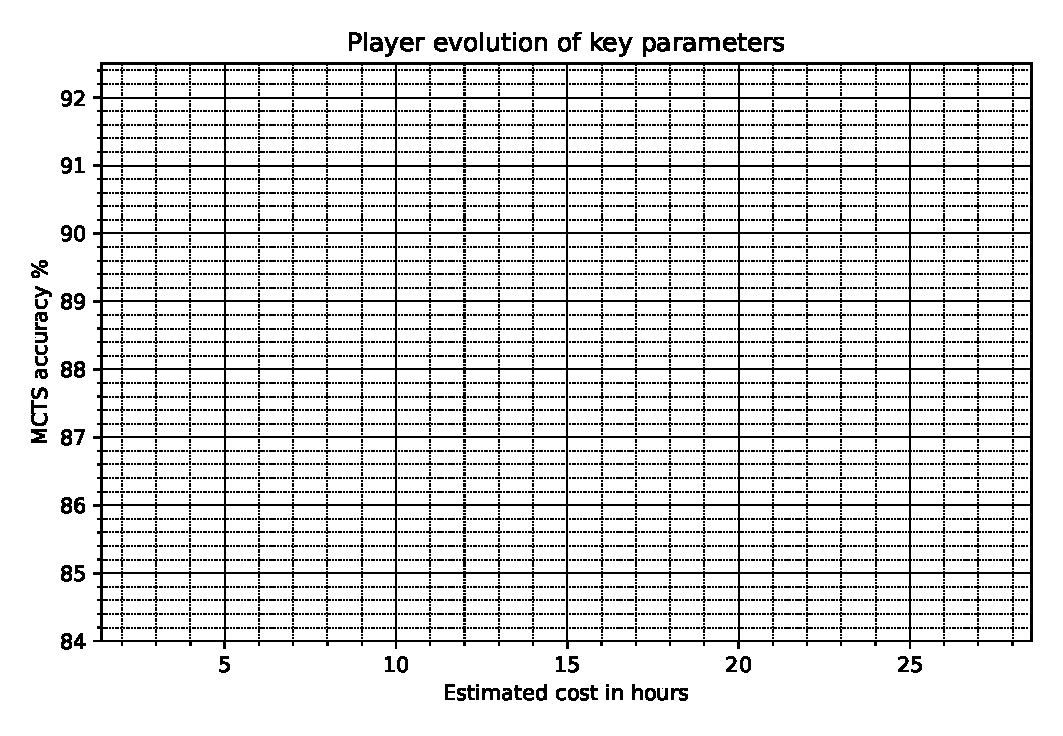
\includegraphics[scale=0.625]{evolve_results0}}
\only<2>{\center 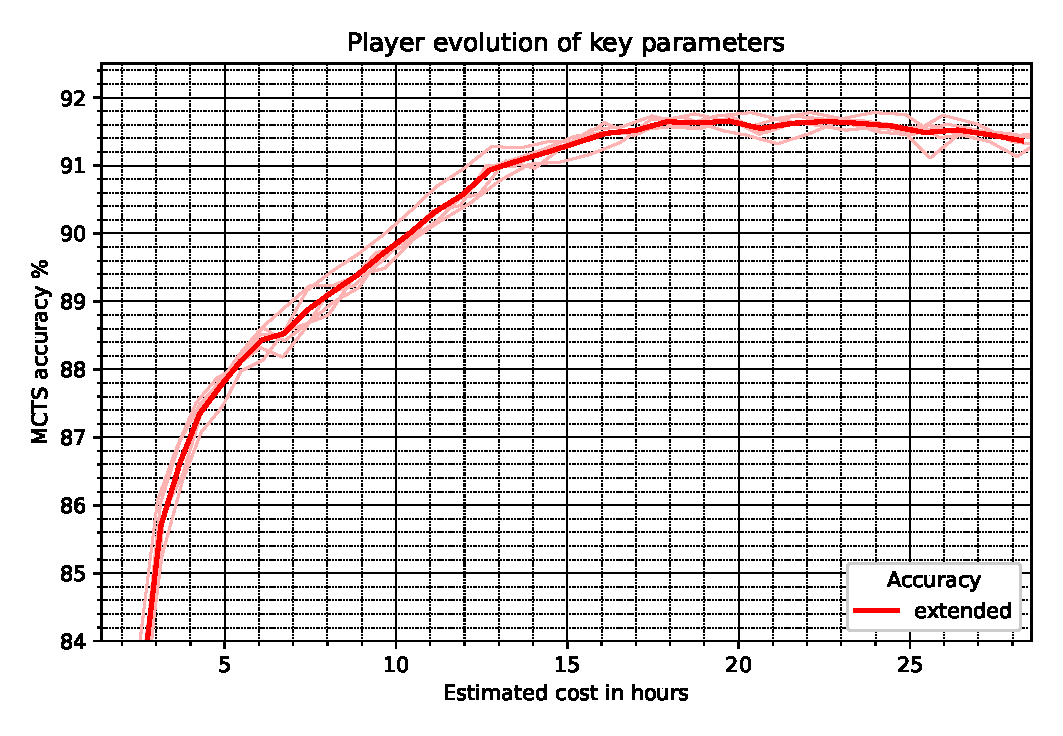
\includegraphics[scale=0.625]{evolve_results1}}
\only<3>{\center 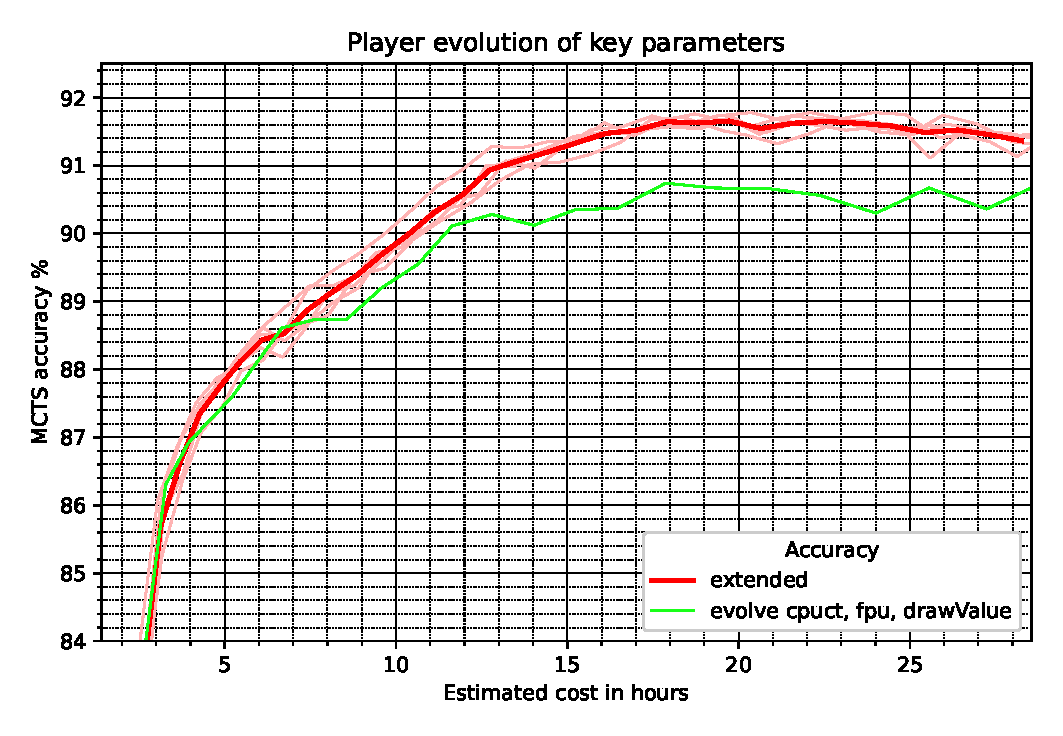
\includegraphics[scale=0.625]{evolve_results2}}
\only<4>{\center 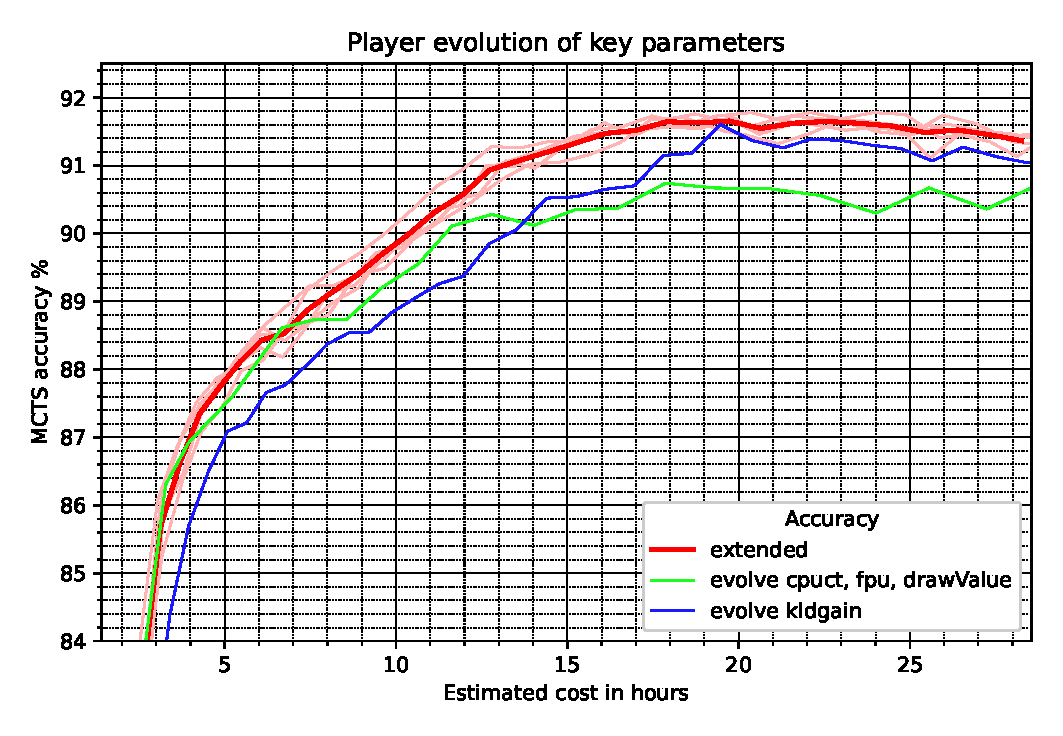
\includegraphics[scale=0.625]{evolve_results}}

  
\end{frame}
\begin{frame}
 \frametitle{Untersuchung}
  


\begin{itemize}
  \item \pause Bedingungen für erfolgreiche Evolution:
\begin{itemize}
  \item \pause Die Liga muss gute Parameter erkennen
  \item \pause Viele Siege müssen sich übertragen auf schnelleren Lernfortschritt
\end{itemize}
\end{itemize}

  
\end{frame}
\begin{frame}
 \frametitle{Erkennt die Liga gute Parameter?}
  


\begin{itemize}
  \item \pause "Gut" im Sinne der Evolution: Gewinne viele Spiele
  \item \pause Erfinde einen neuen Parameter für den der optimale Wert klar ist
  \item \pause Stelle die Bewertung der Spielzüge auf den Kopf.
  \item \pause Wertebereich von 0 bis 1.
\begin{itemize}
  \item \pause Bei 0 hat der Parameter keinen Effekt
  \item \pause Bei 1 werden gute Züge selten gespielt, schlechte am häufigsten.
\end{itemize}
\end{itemize}
\pause \center 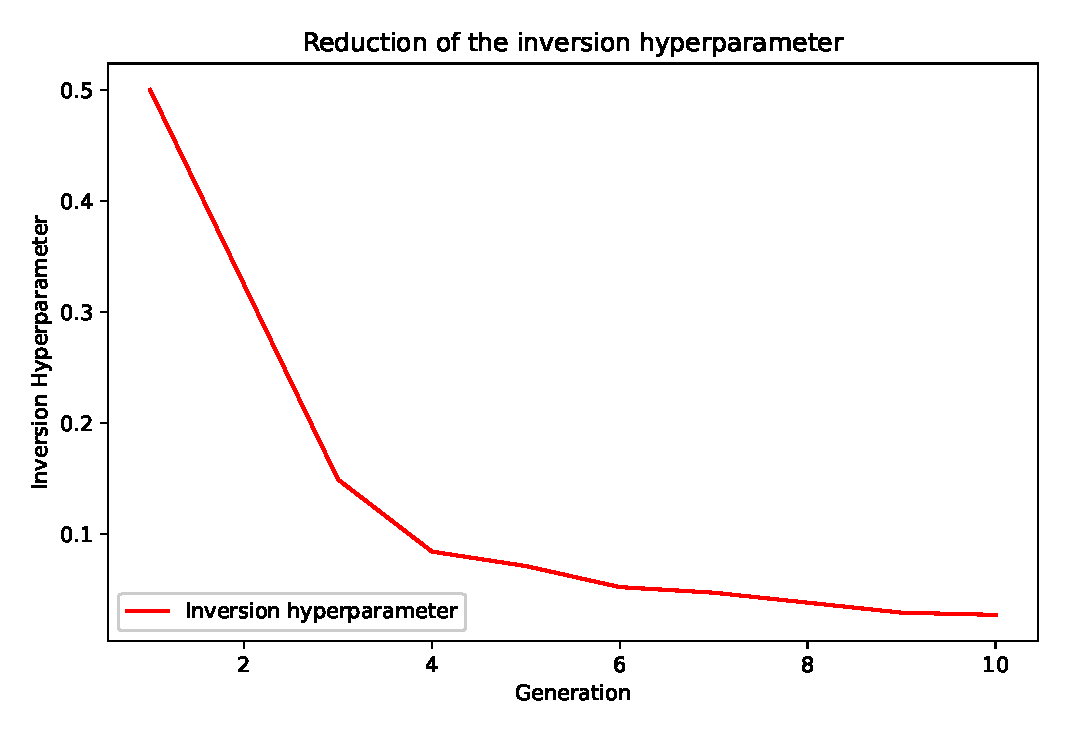
\includegraphics[scale=0.3]{inversion_reduction}
\begin{itemize}
  \item \pause Ein voller Trainingslauf hat eher 30 bis 50 Generationen
  \item \pause Die Liga mit Evolution funktioniert
\end{itemize}

  
\end{frame}
\begin{frame}
 \frametitle{Folgt Lernfortschritt aus mehr Siegen?}
  


\begin{itemize}
  \item \pause Lernfortschritt bedeutet höhere Übereinstimmung mit dem Solver
  \item \pause Vergleiche 3 Hyperparametersets
\begin{itemize}
  \item \pause Bester Spieler aus der Evolution
  \item \pause Baseline Parameter
  \item \pause Bayesian Optimization
\end{itemize}
  \item \pause Vergleiche die 3 Optionen in 1000 Spiele Matches
\end{itemize}

  
\end{frame}
\begin{frame}
 \frametitle{Folgt Lernfortschritt aus mehr Siegen?}
  


\pause
\begin{table} [H]
 \centering

  \begin{tabular}{ c c c c }
  \\
	Evolved Player vs...       &   \\
  \hline
  Baseline & 557W, 155L, 228D \\
  Bayesian Opt. & 442W, 388L, 190D  \\
  \end{tabular}

\end{table}

\begin{itemize}
  \item \pause Klarer Sieger: Die Evolution
  \item \pause Viele gewonne Spiele bedeuten also nicht hoher Lernfortschritt
  \item \pause Nach hoher Siegesrate zu optimieren ist also nicht zielführend
  \item \pause Eine weitere untersuchte Alternative: Novelty search
\begin{itemize}
  \item \pause Keine bedeutend höhere Diversität.
  \item \pause Die Hyperparametersuche hat darauf schon implizit geachtet
\end{itemize}
\end{itemize}

  
\end{frame}

\subsection{Games as trees}



\begin{frame}
 \frametitle{Implementierung: Games as trees}
  


\begin{itemize}
  \item \pause Exploration durch Zurücksetzen an kritische Positionen
  \item \pause Spiele als MCTS-Baum
  \item \pause Notwendigkeit für MCTS-Evaluation Service
  \item \pause Nebeneffekt: Keine doppelte Auswertung von Positionen
\end{itemize}
\only<6>{\center 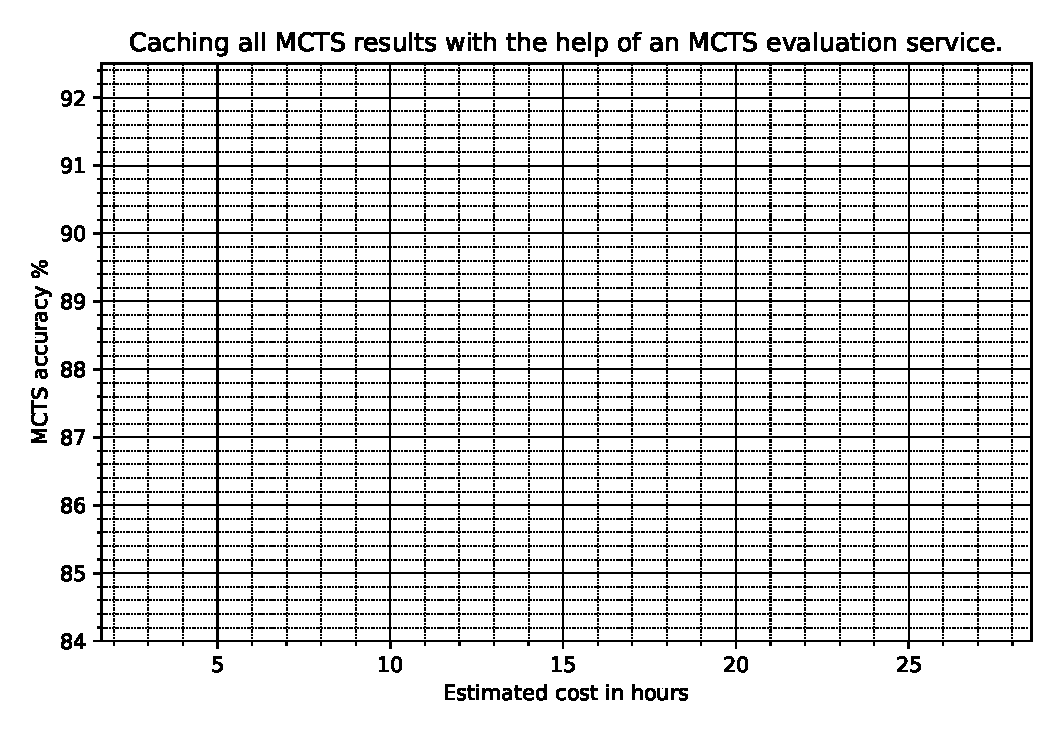
\includegraphics[scale=0.425]{cache_play0}}
\only<7>{\center 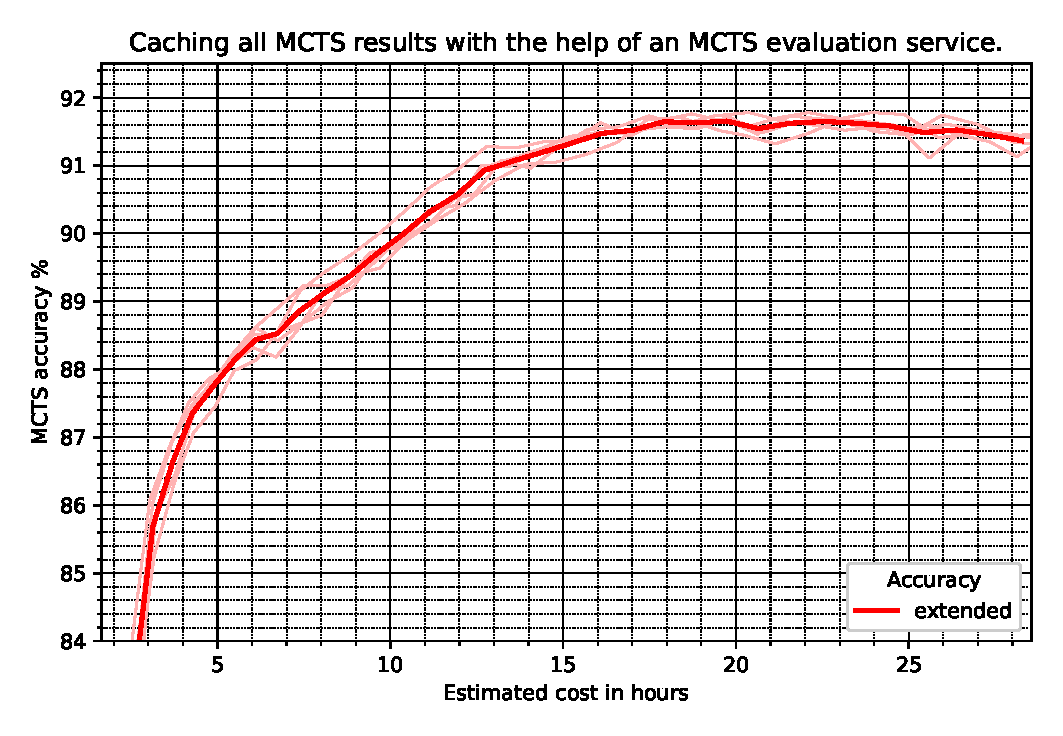
\includegraphics[scale=0.425]{cache_play1}}
\only<8>{\center 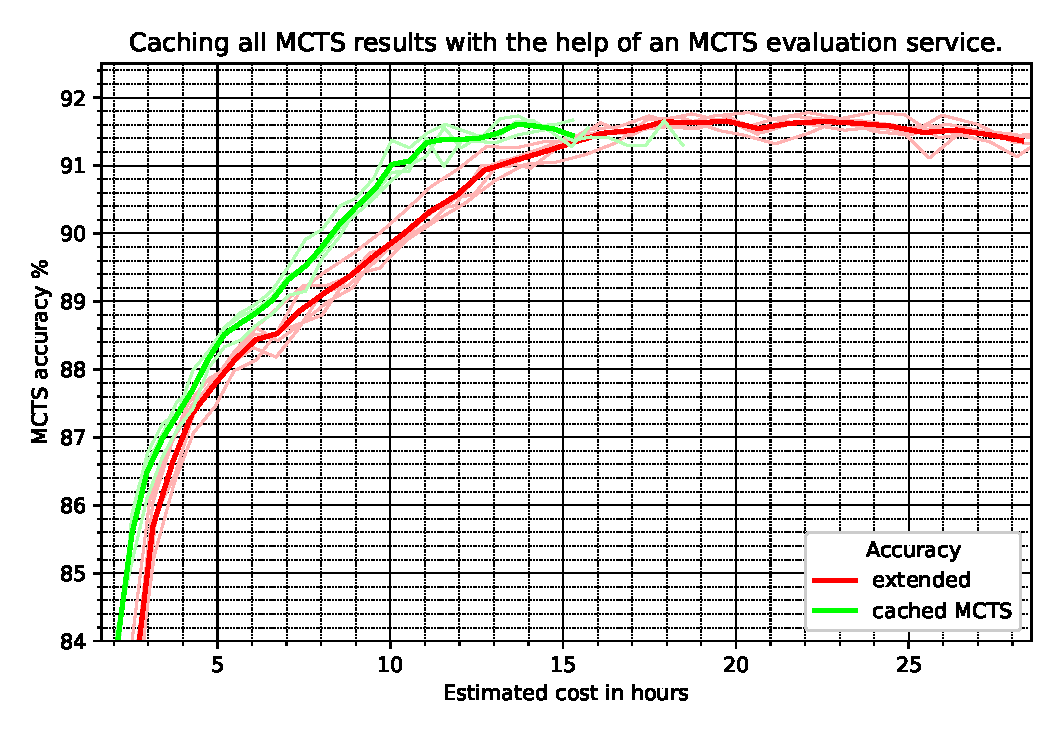
\includegraphics[scale=0.425]{cache_play}}


  
\end{frame}
\begin{frame}
 \frametitle{Zurücksetzen auf kritische Position}
  


\begin{itemize}
  \item \pause Nach einer Niederlage darf der Verlierer einen Zug zurücknehmen
  \item \pause Wähle Position anhand der Entwicklung der Positionsevaluation
  \item \pause Beginne neues Spiel in dieser Position
\end{itemize}
\only<5>{\center 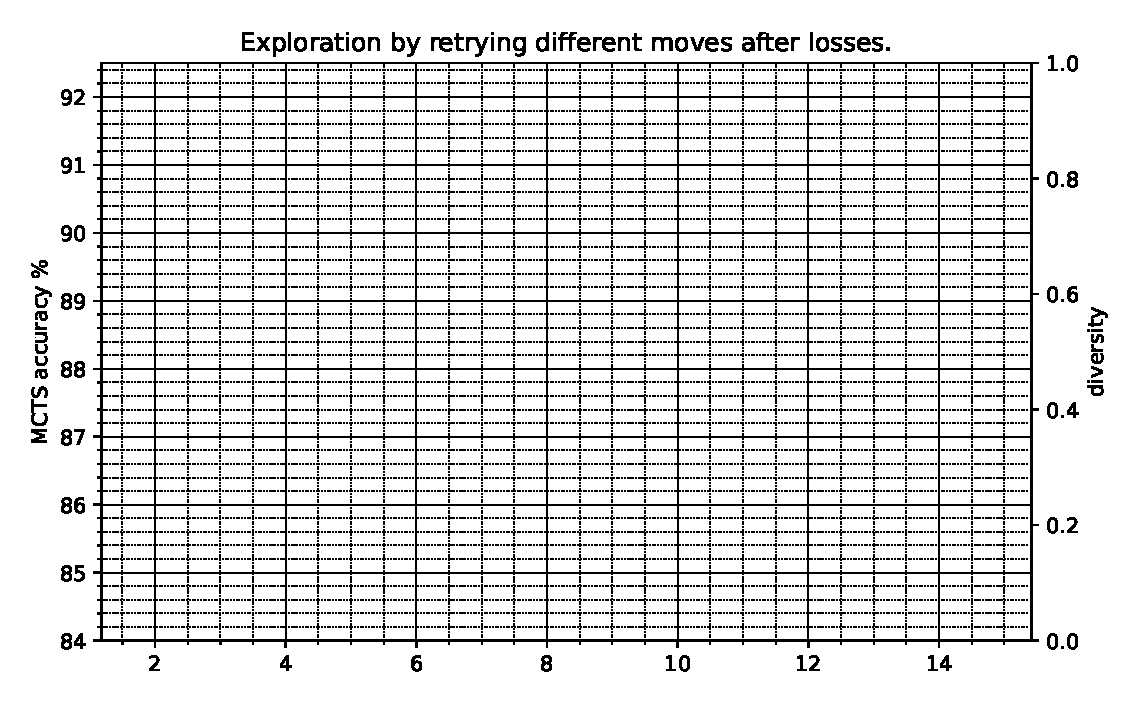
\includegraphics[scale=0.425]{winp_tree0}}
\only<6>{\center 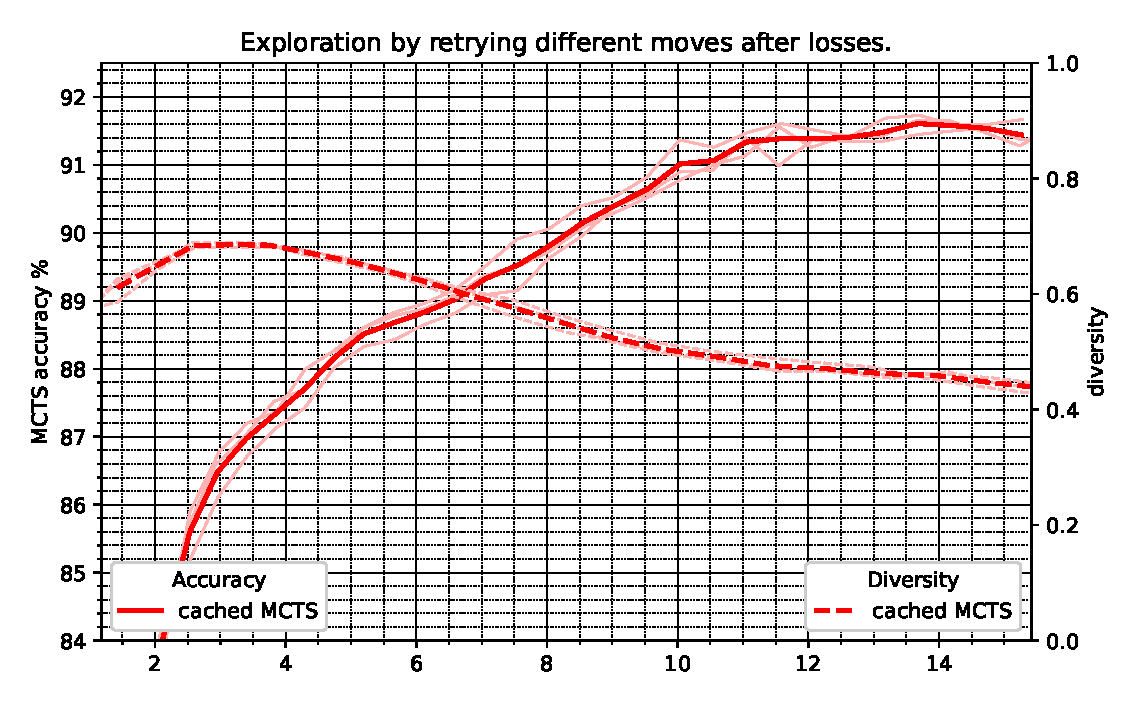
\includegraphics[scale=0.425]{winp_tree1}}
\only<7>{\center 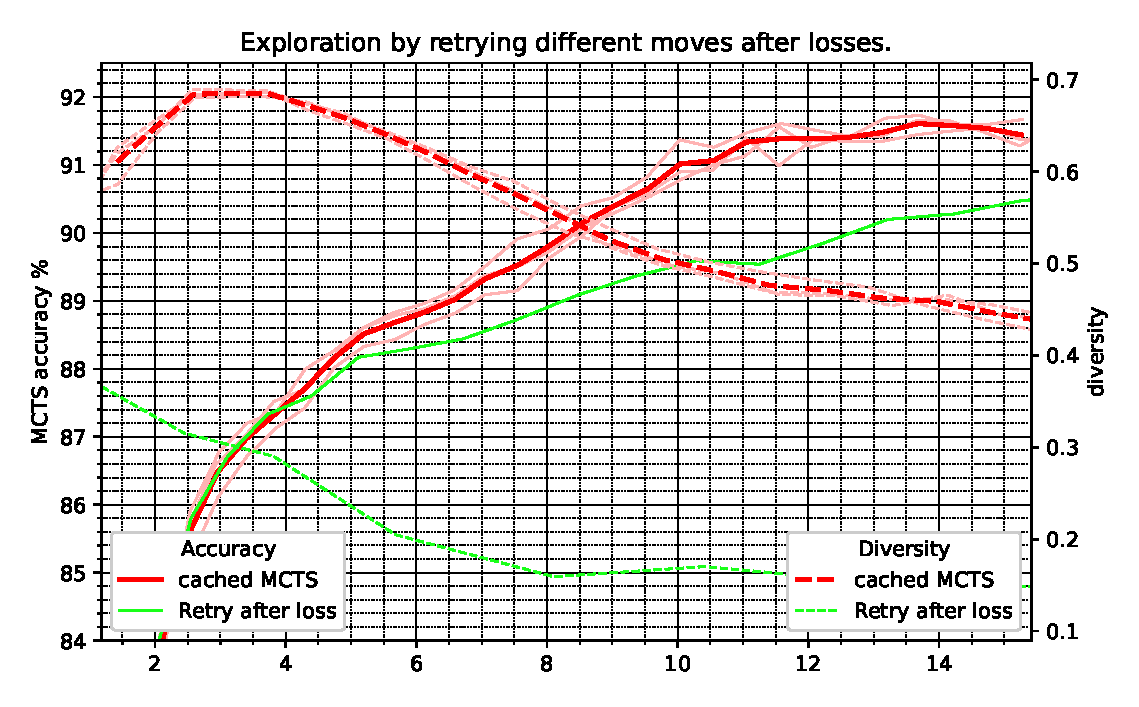
\includegraphics[scale=0.425]{winp_tree}}

  
\end{frame}
\begin{frame}
 \frametitle{Spiele als MCTS-Baum}
  


\begin{itemize}
  \item \pause Exploration-Exploitation: MCTS macht das
  \item \pause Baue einen einzigen MCTS Baum
\begin{itemize}
  \item \pause 150k+ Knoten
\end{itemize}
  \item \pause Reporte die Positionen in den Knoten als Trainingspositionen
\end{itemize}
\only<5>{\center 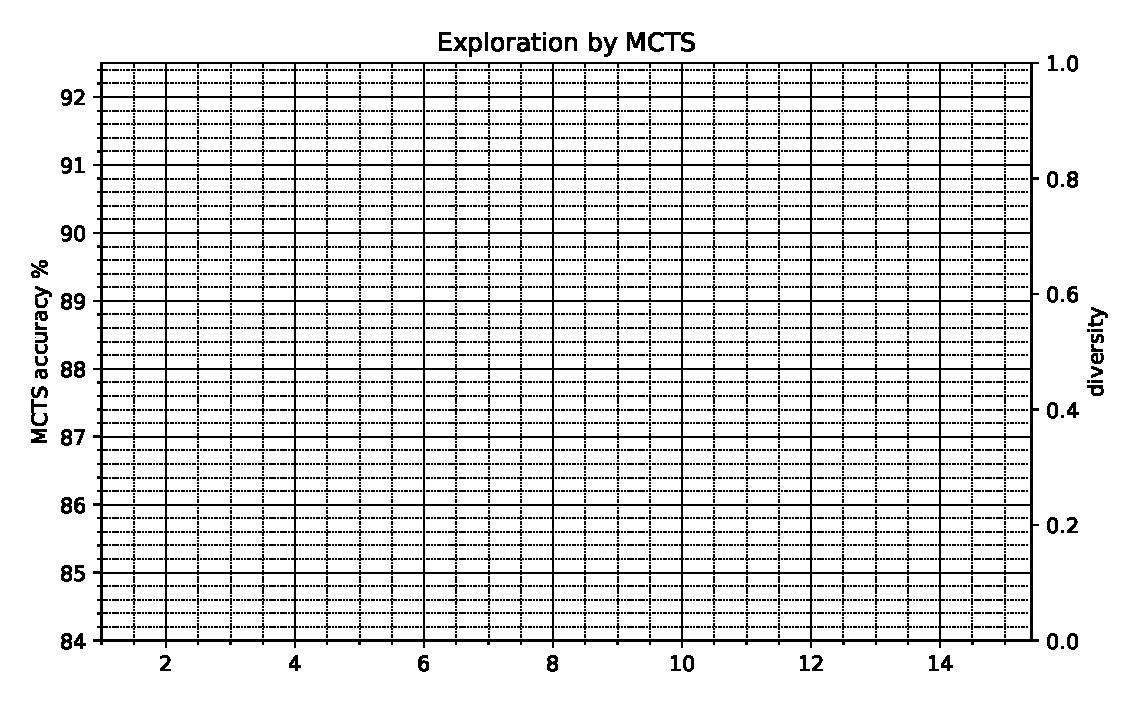
\includegraphics[scale=0.425]{mcts_tree_explore0}}
\only<6>{\center 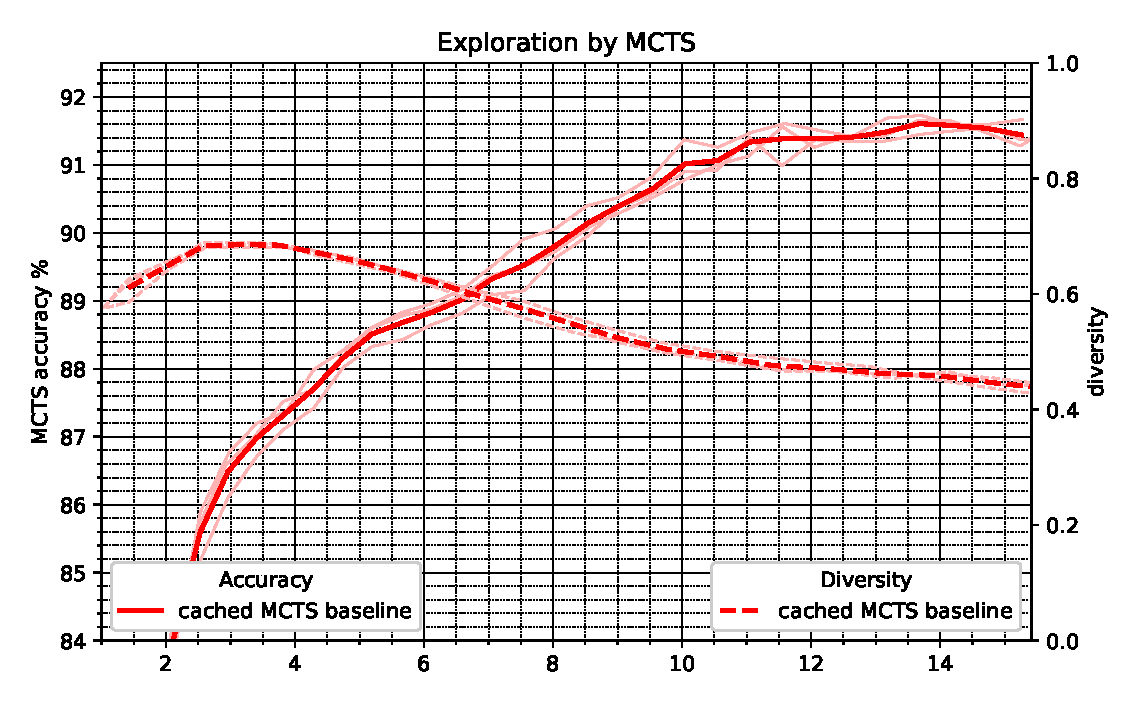
\includegraphics[scale=0.425]{mcts_tree_explore1}}
\only<7>{\center 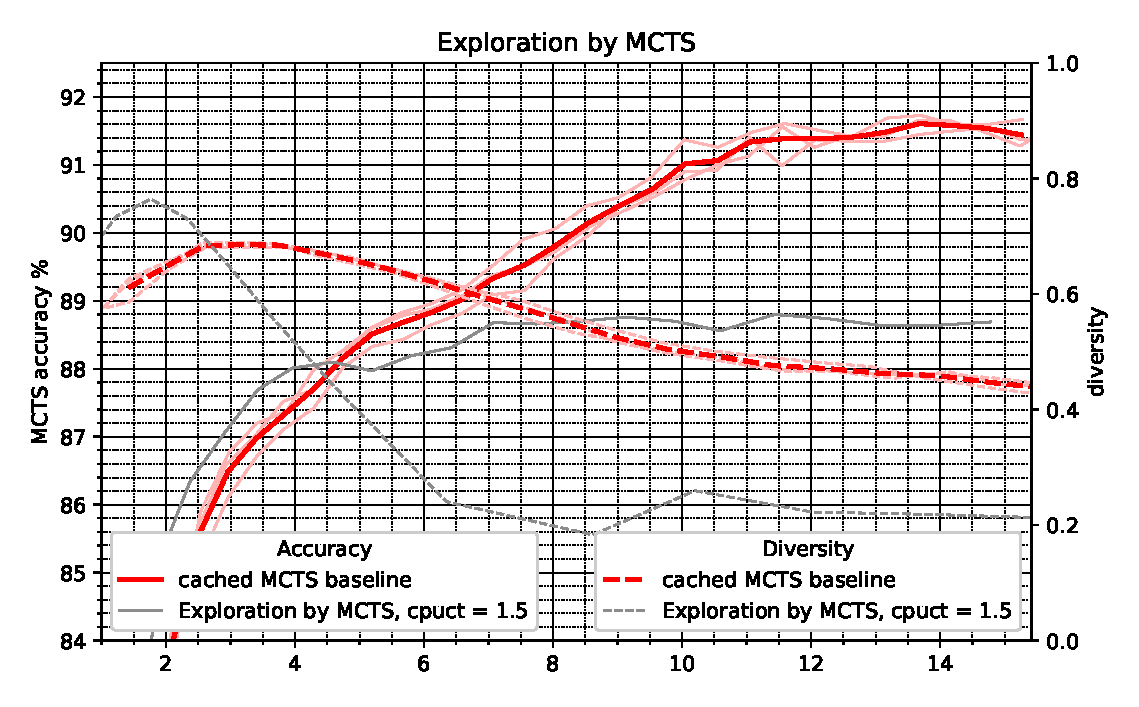
\includegraphics[scale=0.425]{mcts_tree_explore2}}
\only<8>{\center 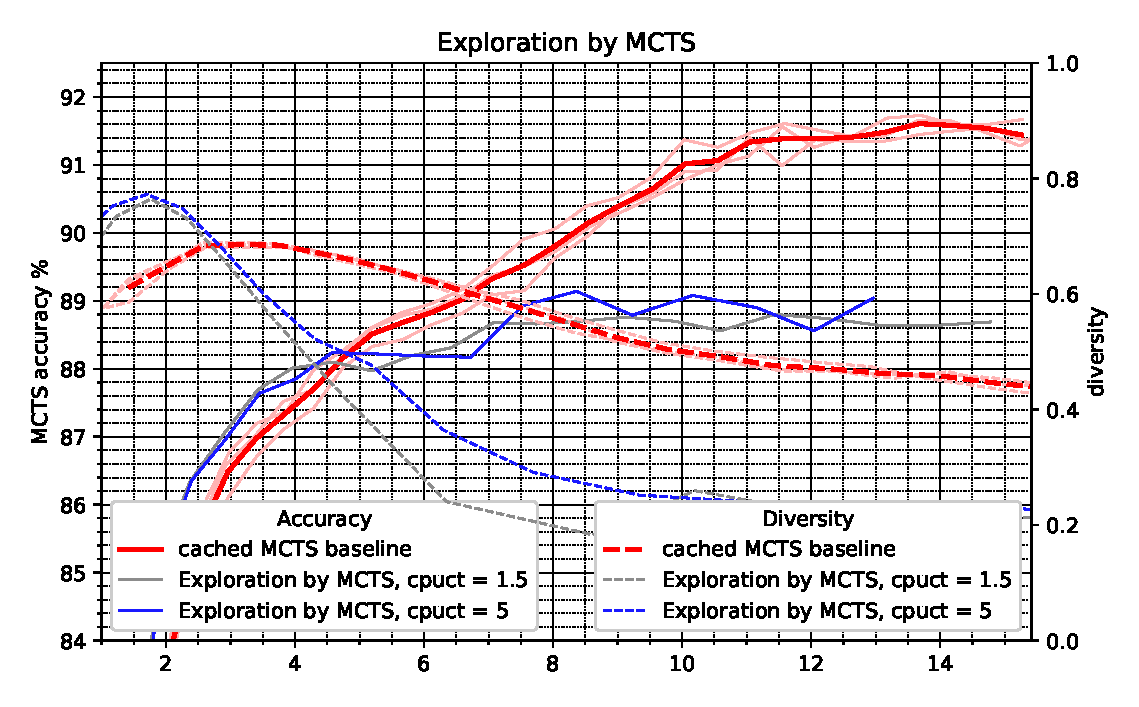
\includegraphics[scale=0.425]{mcts_tree_explore3}}
\only<9>{\center 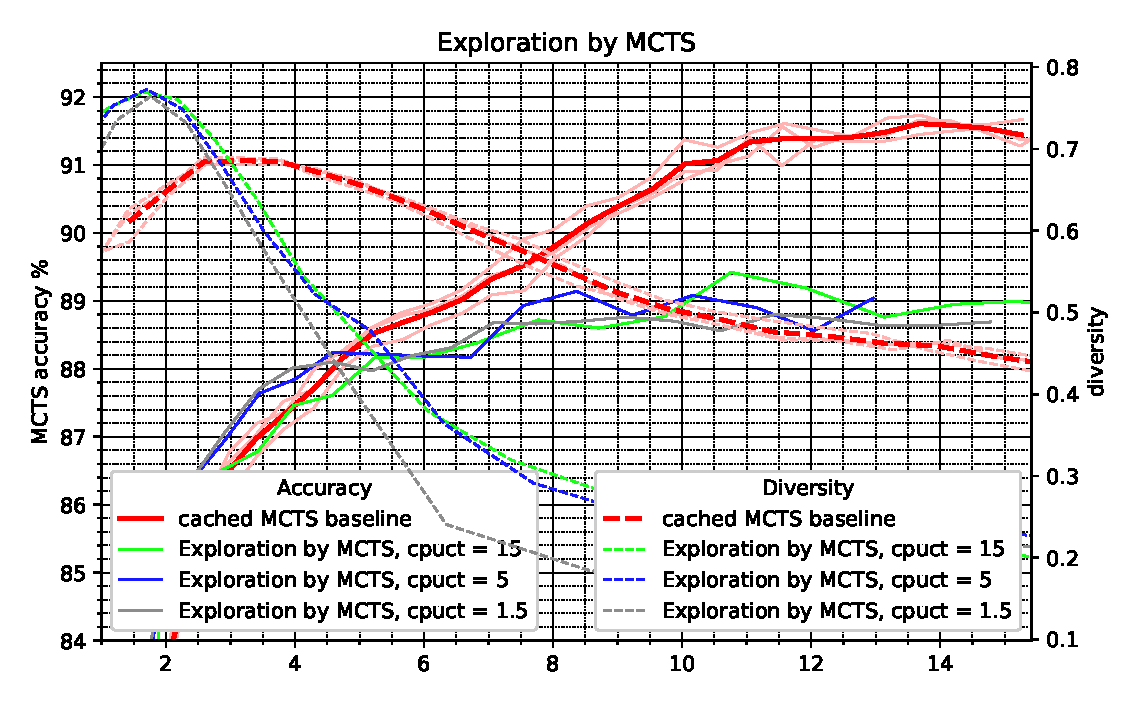
\includegraphics[scale=0.425]{mcts_tree_explore}}

  
\end{frame}

\subsection{Auxiliary features}



\begin{frame}
 \frametitle{Implementierung: Auxiliary features}
  


\begin{itemize}
  \item \pause Trainiere ein kleines Netzwerk, ca. 70k Parameter
  \item \pause Verwende interne Features aus diesem Netzwerk zur Regularisierung des großen Netzwerkes
  \item \pause Verschiedene Optionen wurden im Supervised Setting vorselektiert
  \item \pause Kleine Gewinne im Supervised Setting, keine Gewinne im AlphaZero Setting
\end{itemize}

  
\end{frame}
\begin{frame}
 \frametitle{Untersuchung}
  


\begin{itemize}
  \item \pause Positiver Effekt auf initialen Anstieg der Spielstärke
  \item \pause Negativer Effekt auf finale Spielstärke
  \item \pause Ein zufälliges Netzwerk zeigt diesen Effekt deutlich weniger
  \item \pause Kosten des Trainings des kleinen Netzwerkes sind zu hoch.
  \item \pause Zwei Probleme mit dem Ansatz:
\begin{itemize}
  \item \pause Trainingskosten des kleinen Netzwerks
  \item \pause Finale Spielstärke wird gestört
\end{itemize}
\end{itemize}

  
\end{frame}
\begin{frame}
 \frametitle{Untersuchung}
  

\only<1>{\center 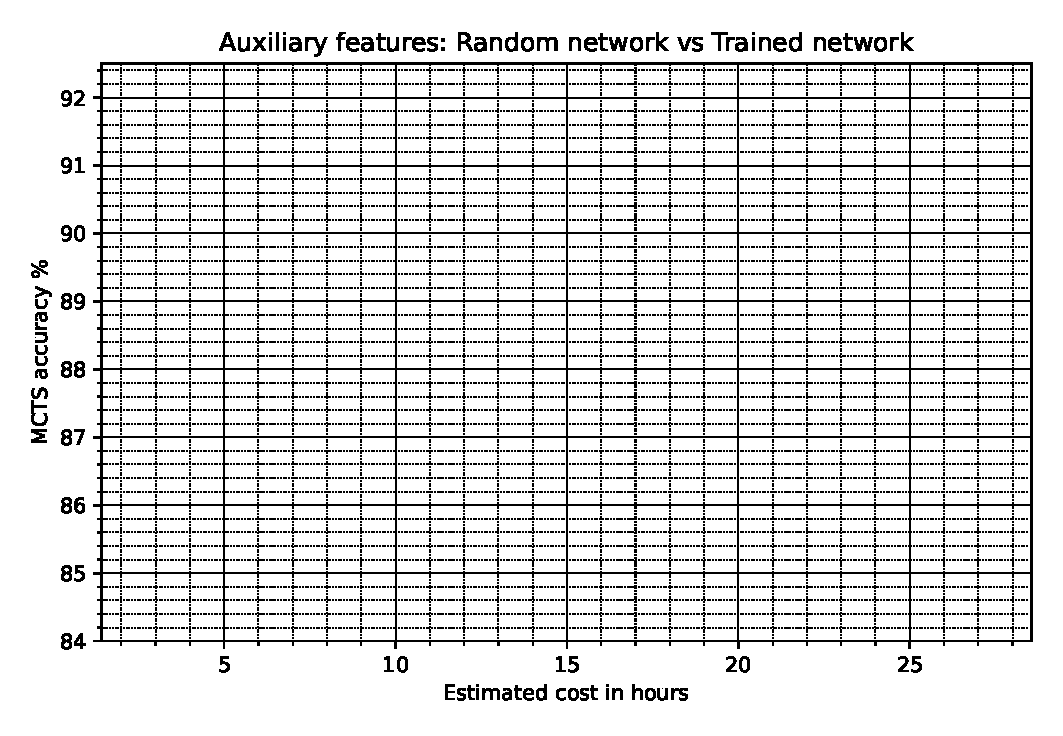
\includegraphics[scale=0.425]{rndVsTrainedAux0}}
\only<2>{\center 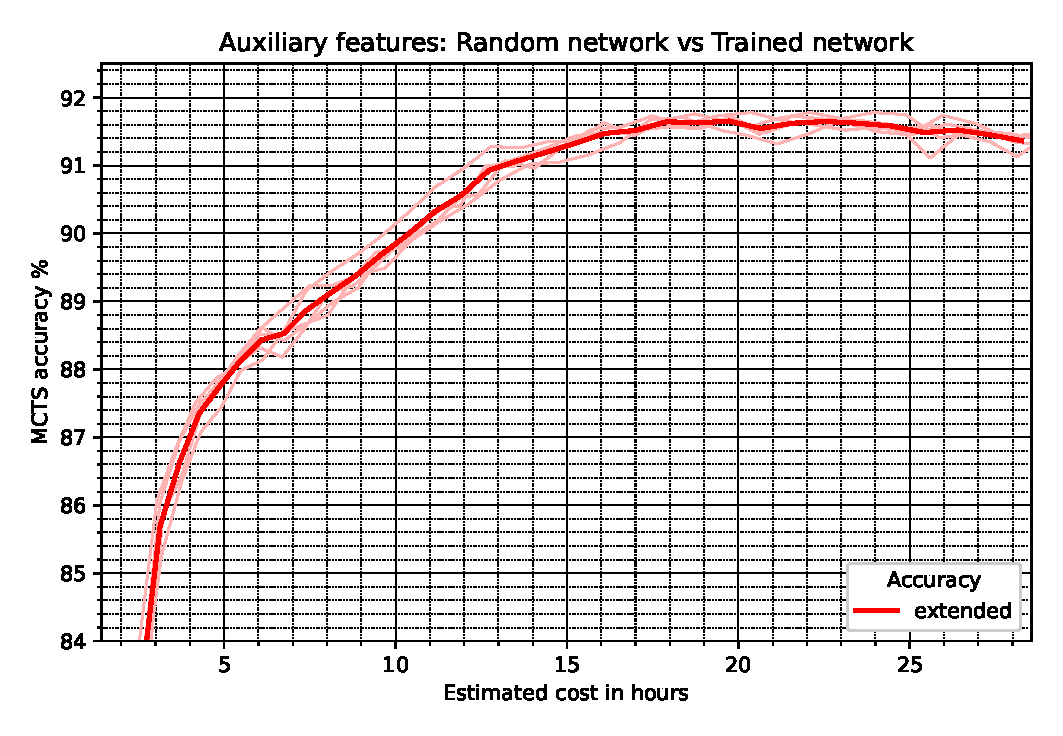
\includegraphics[scale=0.425]{rndVsTrainedAux1}}
\only<3>{\center 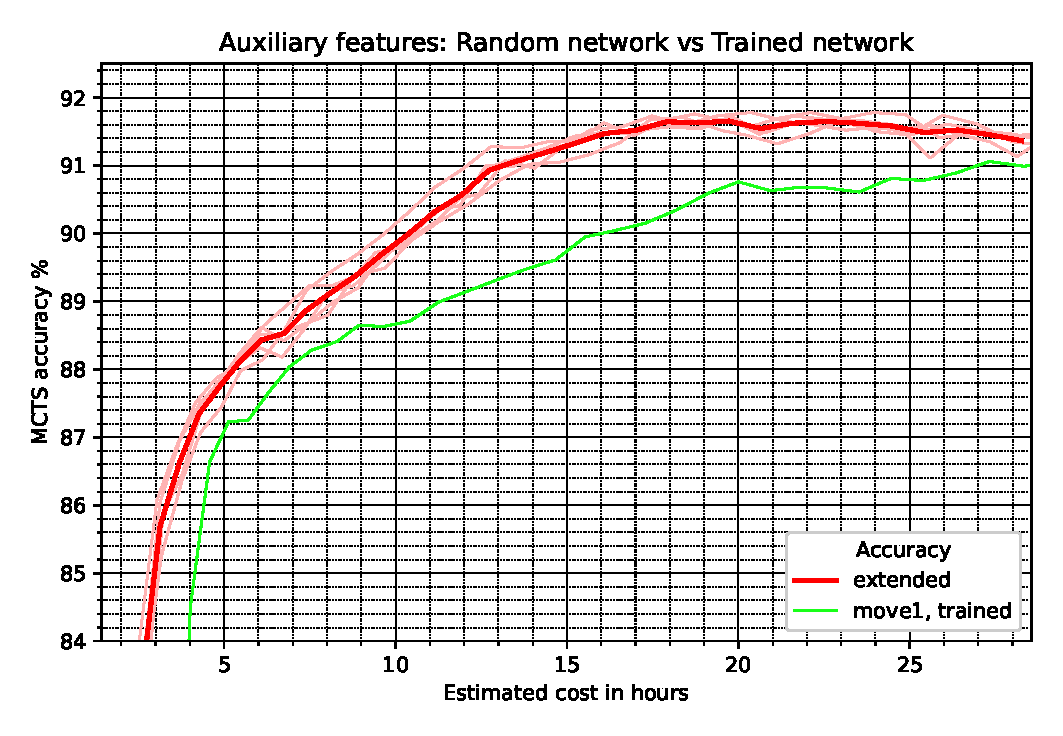
\includegraphics[scale=0.425]{rndVsTrainedAux2}}
\only<4>{\center 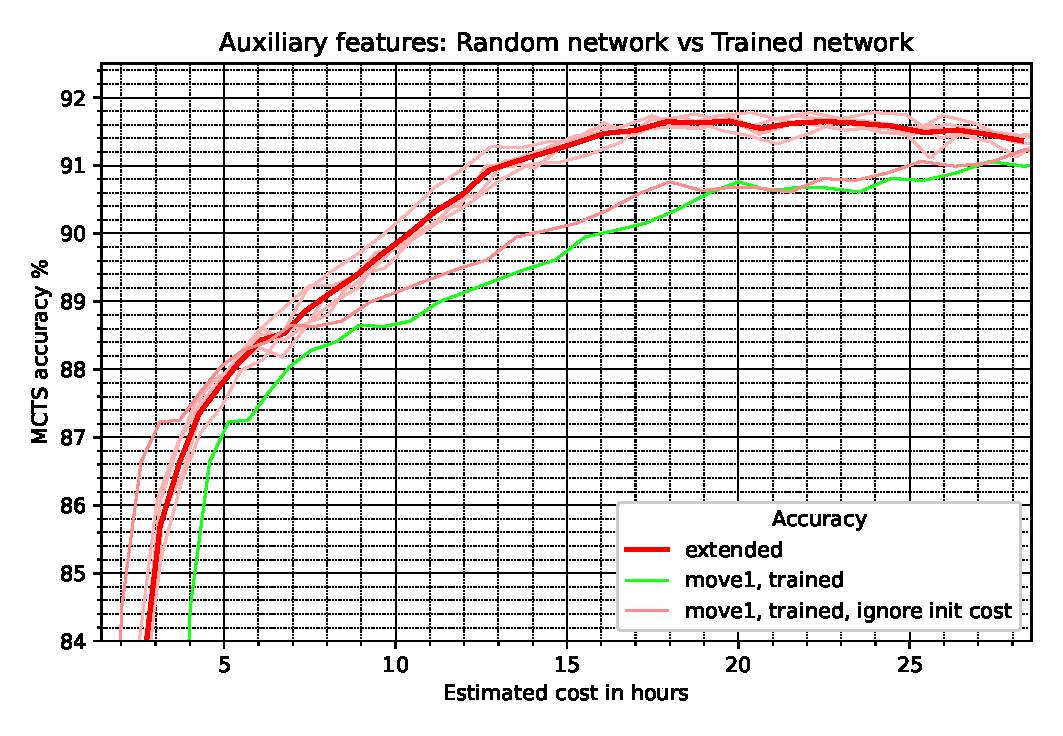
\includegraphics[scale=0.425]{rndVsTrainedAux3}}
\only<5>{\center 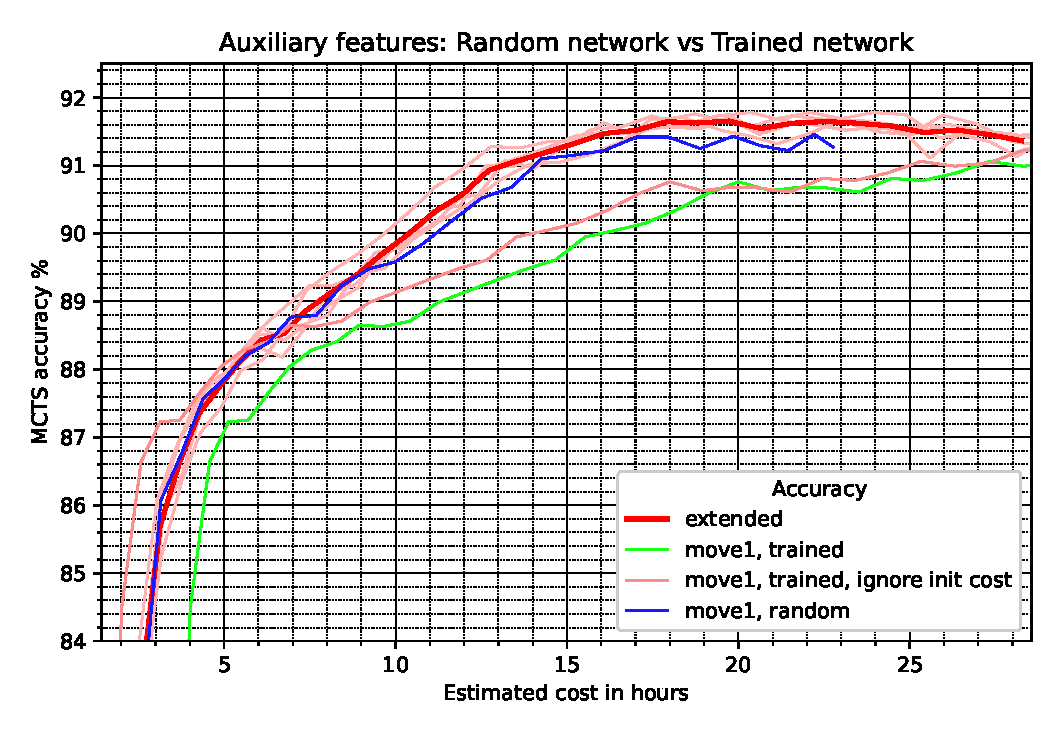
\includegraphics[scale=0.425]{rndVsTrainedAux}}


  
\end{frame}
\begin{frame}
 \frametitle{Das Netzwerk wachsen lassen}
  


\begin{itemize}
  \item \pause Beginne den AlphaZero Trainingslauf mit kleinem Netzwerk
  \item \pause Tausche des Netzwerk alle paar Iterationen gegen größeres aus
  \item \pause Dieses Vorgehen ist generell effektiver
  \item \pause Aber keine neue Idee
  \item \pause Die Trainingskosten des kleinen Netzwerkes verschwinden
\end{itemize}

  
\end{frame}
\begin{frame}
 \frametitle{Finale Spielstärke darf nicht geschadet werden}
  


\begin{itemize}
  \item \pause Auxiliary features dürfen nicht der finalen Spielstärke schaden
  \item \pause Es wurden verschiedene Optionen erprobt
  \item \pause Keine verbesserte die Situation
\end{itemize}

  
\end{frame}

\subsection{Fazit}



\begin{frame}
 \frametitle{Fazit}
  


\begin{itemize}
  \item \pause AlphaZero Experimentalframework entwickelt
  \item \pause Keine großen Verbesserungen gefunden
  \item \pause Trotzdem einiges Interessante Erkenntnisse
\begin{itemize}
  \item \pause Nicht alle Ideen vorheriger Arbeiten funktionieren mit Vier gewinnt
  \item \pause Evolution für Hyperparameter funktioniert
\begin{itemize}
  \item \pause Nur eine gute Fitnessfunktion fehlt
  \item \pause Unterschied zwischen Lernfortschritt und Spielstärke
\end{itemize}
  \item \pause Alternative Explorationsmethoden zeigen vor allem wie gut die einfache Standardversion funktioniert
  \item \pause Auxiliary features aus dem inneren eines kleineren Netzwerks sind nur schwer nutzbar
\begin{itemize}
  \item \pause Aber das Konzept des Netzwerkwachstums sollte weiter erforscht werden
\end{itemize}
\end{itemize}
\end{itemize}


  
\end{frame}

\section{Ende}



\begin{frame}
 \frametitle{Referenzen}
  


\centering Danke für Ihre Aufmerksamkeit.


\begin{itemize}
  \item Maybe do some references here...
\end{itemize}



  
\end{frame}

